% ============================================================
%  第五卷 第六章 凝聚体（§64–§73 + 习题）
%  底本：高教社中文版第5版；OCR 底稿 full_merged.md 行 6933–7990
%  插图：图8（§66，C/(3Nν)–T/Θ 曲线）、图9（§70，鞍点等频面）、
%        图10（§73，负温度的 S(E) 曲线）；图11 在第七章区间（OCR 行 8089）
%
%  已修正的 OCR/原书错误（除注明外均对照原书页面 PNG 核验）：
%   [§64] (64.3) 与平均声速定义式原书均误印 u_l（p173），按纵/横波偏振数
%         物理意义订正为 1/u_l^3 + 2/u_t^3 与 2/u_t^3 + 1/u_l^3；
%         (64.7) (ħπ)^3→(ħū)^3；S 的乱码下标→S_0、TS_∘→TS_0；
%         "原子C和0"→C和O；3Nv→3Nν、ε_∘/N_𝔈₀→ε₀/Nε₀ 多处；
%         "与物体的温度无关"后补冒号 ε₀=ε₀(N/V)；s∝T³→S∝T³（p174 大写）；
%   [§65] (65.9) dT→dΓ；"从−∞ 𝔈𝔥 +∞"乱码→到；F_onh→F_anh（(65.11)）；
%         N_{E_0'}→Nε₀'；T_∥→T₁（习题1）；\widehat{f}₂→f₂（p176 无帽）；
%   [§66] "图8给出"→"图8给出了"（照 p178 原书）；(66.1) u→ū（补平均号）；
%         θ 与 Θ 混排统一为 Θ；\daleth 乱码删除；
%   [§67] "正比于T₃"乱码→正比于T；α 式中 V₀𝒞²→V₀Θ²；c=−(T/θ)f″→C；
%   [§68] "(..，1952)"→（И. М. Лифшиц, 1952）按 p182 还原作者名；
%         "常数·T²/(u₄γ)"之 OCR 乱码按 p183 还原；"可略 κ* 项"→κ⁴；
%         T^{s/2}→T^{3/2}（(68.9)）；k_*→k_z 多处；(68.5)(68.6)(68.7)(68.9)
%         中乱码 arg/∃/∧/LF→"当…时"按 p183–184 还原；
%   [§69] 力学系数记号 A/λ 混排统一为 Λ（照 p185–186，正文亦作"系数Λ"）；
%         (69.5) 求和指标 n′→n；(69.9) S_{ik}S_{is′}→δ_{ik}δ_{ss′}；
%         (69.10) 中间项上标 s′s 按 p185 缩放还原（照原书中间项无 * 号）；
%         "振动谱支1"→谱支①；"基本周期†"之 † 系 OCR 噪声，原书无
%         （脚注圈码①在"是整数"括号后，p186）；(69.15) f(k/k)；
%   [§70] (70.7) 乱码 ω/ħ·ω/𝒦·ω²→常数·ω²（照 p189，带编号 (70.7)）；
%         "色散关系形为(69.5)"→(69.15)：原书排印误——(69.5) 为 ΣΛ(n)=0，
%         声学振动的色散关系是 (69.15)（英译本同此）；
%         (70.9) 首行 g(ω₀)=…→g(ω₀)−…（负号，照 p190 原书）；
%         √[3]γ→√γ、积分上限 x→K、x₁,x₂,φ→κ_⊥,κ_z,φ；\mathfrak{O}→①；
%   [§71] h→ħ 多处（p190–192 均作 ħ）；"引人"→引入；\mathcal{Q}_S 乱码→②
%         （p191 确认圈码②在"k 值进行"后）；(71.4) ħb′；
%   [§72] (72.1)(72.15) e^{ik·r_s}→r_n；(72.2) m=Σm→m=Σm_s；
%         (72.6) 求和下标还原为 ns 与 nn′,ss′（p193）；
%         哈密顿方程句"就是 Ṗ=Q̇"→"就是 P=Q̇"（照 p194）；
%         (72.15) 根式 ħ/2mN→ħ/(2mN)；
%   [§73] E_*/Ē_*→E_n/Ē_n（下标 n）；Z_ms→Z_mag；t_!→t₁；\mathfrak{D}→①；
%   [全章] \mathrm{d} 收紧；\sin\ln\exp\det 等函数名统一；e、i 用正体；
%         页界断行/断段合并多处；显示式末标点按原书照排.
%
%  遗留问题：
%   - 脚注已全部转录完毕（共 31 处 \footnote，圈码已删；对照原书 pages300
%     p185–p194、p196–p203、p206–p207、p209–p212 逐一核验；p192/193/195/
%     204/205/208/211 无脚注；§73 脚注①圈码在 p212 首行"降（图10）①"，
%     脚注页码对照.txt 记 p211 系 ±1 页界偏差）：
%     §64 p185①、p186①（量子晶体，Андреев/Лифшиц ЖЭТФ 1969）、p187①（Einstein 1907）
%     ②（参看(71.7)）、p188①（三支声波谱支）、p189①（电子自由度/晶格部分）；
%     §65 p190①（参看§31节末尾）、p191①（A>0）；§66 p194①②③④（D(x) 渐近
%     展开、C 高温下一项、Θ 值表）；§68 p197①（弹性模量式与"小模量"清单：
%     300dpi 扫描件上下标已到分辨极限，按物理与六方对称性读出）②③、
%     p198①②、p199①（链方向小模量清单，同上读法）；§69 p200①（权重因子
%     m_s）、p201①（参看§133）、p202①（k=0 方程）②（Лифшиц/Косевич 文献）、
%     p203①（6 个鞍点）；§71 p206①（折返过程）②；§72 p207①、p209①②
%     （零点能）、p210①；§73 p210②、p212①（S(E) 曲线对称性）；
%   - §68 估计式"ħuκ∼ħu(T/ħγ)^{1/2}"之 u 照原书 p183 排印不带下标
%     （英译本作 u₃），未改；
%   - (69.10) 中间项照原书无复共轭号（按数学关系疑脱 *，照排，p185）；
%   - §64"假设物体是各向同性的(非晶固体)"、§72"可用过不同数目的声子
%     生成算符和湮没算符的乘积表示"均系原书原貌（p172/p195），照排.
% ============================================================
\chapter{凝聚体}

\section{低温下的固体}

能够有成效地应用统计方法来计算热力学量的另一类对象是固体.固体的特征在于：其中的原子仅仅在某些平衡位置——晶体的格点——附近作微小的振动.对应于物体热平衡的格点间相互配置是选定的，即是有别于所有其它可能的分布，因而是规则的.换句话说，在热平衡状态下的固体应该是晶体.

根据经典力学，在绝对零度下原子是不动的，它们的相互作用势能应该取平衡极小值.因而在足够低的温度下，原子应该总是只作微小的振动，即所有的物体都应该是固态的.然而，在现实中量子效应可以使这个规则产生例外.液氦就是一例，它是在绝对零度(不太高的压强下)仍然保持液态的唯一物质；其它所有物质早在其中的量子效应变得重要以前就已经固化了\footnote{当与原子的热运动相对应的德布罗意波长变得可以同原子间距相比较的时候，量子效应变得重要. 在液态氦中，这种情况在 $2\sim3\,\mathrm{K}$ 时开始出现.}.

要使物体成为固体，它的温度与原子相互作用能相比在任何情况下应该很小(事实上在较高的温度下所有的固体都已经熔化或分解).与此相关，固体中的原子在它们的平衡位置附近的振动总是很小的.

在自然界中除晶体外还存在着一种非晶固体，其原子在混乱排列的点附近振动.从热力学的观点来看，这种物体是亚稳定的，随着时间的推移终究会结晶的.但是事实上，它们的弛豫时间是如此的长，以致在无限长的时间内，非晶体的行为实际上都像是稳定状态的物体一样.下面所有的计算同样地适用于晶体和非晶体.区别仅仅在于：由于非晶体的非平衡性，能斯特定理不适用于它们，T→0 时它们的熵趋向于不等于零的值.因此对于非晶体来讲，对下面所得到的熵的公式(64.7)必须附加某个常数 $S_0$(而对自由能必须附加相应的项 $TS_0$)；但是这个不很重要的常数并不影响例如物体的热容，我们将省略掉它.

这种在 T→0 时不等于零的剩余的熵在晶态固体中也可以观测到，这与所谓的晶体有序化现象有关.一种给定类型的原子可以出现在晶体格点上，如果格点数同该类原子的数目一致，那么在每一格点附近都有一个原子；换句话说，在每一格点附近出现该种类型的任何一个原子的概率等于一.这样的晶体称为完全有序的.但是，也存在着这样的晶体：在这种晶体中原子不仅可能出现在它们“自身的”位置(即完全有序时它们所占据的位置)上，而且也可能出现在另一些“他身的”位置上.在这种情形下，可能出现该类原子的格点的数目超过这些原子的数目；显然，这时该类原子出现在无论老的或者新的格点上的概率都不等于一.

例如，固态的一氧化碳是分子晶体，其中分子 CO 可以有两种相反的取向：通过把原子 C 和 O 相互置换的方式就可以从一种取向得到另一种取向；在这种情形下，可能出现原子 C(或 O)的位置的数目是这些原子的数目的两倍.

在绝对零度下的完全热力学平衡状态中，任何晶体都应该是完全有序的，即每一类原子都应该占据完全确定的位置\footnote{严格地说，这个说法仅在忽略量子效应时才正确. 如果晶格原子零点振动的振幅与原子间距可比，量子效应可以变得很重要（在 $T=0$ 时）. 原则上，在这种“量子晶体”中，基态（$T=0$ 的状态）时格点数有可能超过原子数. 于是，晶格中可存在“零点”缺陷（自由空位），但它们并不（像在经典晶体中那样）定位在任何特定的格点上，而表现为不打乱周期性的晶格集体性质. 参看 Андреев А Ф, Лифшиц И М. ЖЭТФ, 1969, 56: 2057.}.但是由于晶格结构重排过程非常缓慢(特别是在低温下)，在高温下不完全有序的晶体，到很低的温度下事实上也可能仍然保持着这种不完全有序的状态.这种无序性的“冻结”导致晶体的熵中出现一项剩余的常数项.例如，在上述的晶体 CO 的例子中，如果分子 CO 以相等的概率取两种取向，那么剩余熵就等于
\begin{equation*}
  S_0=\ln 2.
\end{equation*}

设 N 是晶格的单胞数，ν 是一个单胞中的原子数.于是原子的总数为 $N\nu$.在总共 $3N\nu$ 个自由度中，三个相应于物体整体的平动，三个相应于物体整体的转动.因此振动的自由度数为 $3N\nu-6$；但是由于 $3N\nu$ 数量非常巨大，当然可以忽略掉 6 这个数，而认为振动的自由度数就等于 $3N\nu$.

应当着重指出：在考虑固体时，我们在这里完全不考虑原子的“内部”(电子的)自由度.因此，如果这部分的自由度是重要的话(例如，在金属中就可能是这样)，那么必须注意到下面所有关于固体的热力学量的公式都只是与原子振动有关的那一部分(通常称为“晶格”部分).要得到这些量的总值还必须把电子的部分附加到晶格的部分上去.

从力学的观点来看，具有 $3N\nu$ 个振动自由度的系统可以考虑为 $3N\nu$ 个独立振子的集合，其中的每一个振子相当于一个单独的简正振动.与一个振动自由度相联系的热力学量我们已经在§49中计算过了.以那些公式为基础，我们可以把固体的自由能直接写成\footnote{振动的量子化是首先由爱因斯坦用来计算固体的热力学量的（A.~Einstein, 1907）.}
\begin{equation}
  F=N\varepsilon_0+T\sum_\alpha\ln\left(1-\mathrm{e}^{-\hbar\omega_\alpha/T}\right)
\end{equation}
的形式.求和是对所有的 $3N\nu$ 个简正振动进行的，它们的编号用角标 $\alpha$ 来表示\footnote{该公式的积分表示参看(71.7).}.我们把一项 $N\varepsilon_0$ 附加到对振动的求和上去，$N\varepsilon_0$ 代表物体的全部原子在平衡位置时(更确切地说，在“零点”振动状态)的相互作用能.该项与密度有关，但是与物体的温度无关：$\varepsilon_0=\varepsilon_0\left(\dfrac{N}{V}\right)$.

我们来研究低温的极限情形.当 T 很小时，在对 $\alpha$ 求和的和式中起作用的只是频率很低的项：$\hbar\omega_\alpha\sim T$.但是低频振动不是别的，就是通常的声波.声波的波长与频率的关系为 $\lambda\sim\dfrac{u}{\omega}$，其中 $u$ 是声速.在声波的情形中，波长比晶格常数 a 大得多($\lambda\gg a$)；这就意味着 $\omega\ll\dfrac{u}{a}$.换句话说，为了能够把振动考虑为声波，温度必须满足写成如下形式的条件：
\begin{equation}
  T\ll\frac{\hbar u}{a}.
\end{equation}

假设物体是各向同性的(非晶固体).大家知道，在各向同性的固体中，纵声波(我们用 $u_l$ 代表它的速度)的传播和具有两个独立偏振方向的横波(具有相同的传播速度 $u_t$)的传播都是可能的.这些波的频率同波矢 $\boldsymbol{k}$ 的绝对值由线性关系式 $\omega=u_lk$ 或 $\omega=u_tk$ 联系着.

在声波的频谱中，波矢绝对值位于间隔 $\mathrm{d}\boldsymbol{k}$ 内而具有一定偏振的本征振动的数目为
\begin{equation*}
  V\frac{4\pi k^2\,\mathrm{d}k}{(2\pi)^3},
\end{equation*}
其中 V 是物体的体积.在三种独立的偏振中，令其中的一种为 $k=\dfrac{\omega}{u_l}$，另外其它两种为 $k=\dfrac{\omega}{u_t}$，我们就求出在间隔 $\mathrm{d}\omega$ 内总共具有的振动数目如下：
\begin{equation}
  V\frac{\omega^2\,\mathrm{d}\omega}{2\pi^2}\left(\frac{1}{u_l^3}+\frac{2}{u_t^3}\right).
\end{equation}
根据定义
\begin{equation*}
  \frac{3}{\bar{u}^3}=\frac{2}{u_t^3}+\frac{1}{u_l^3}
\end{equation*}
我们引入一个平均声速 $\bar{u}$.于是表达式(64.3)可以写成形式
\begin{equation}
  V\frac{3\omega^2\,\mathrm{d}\omega}{2\pi^2\bar{u}^3}.
\end{equation}
在这样的形式下，它不仅可以应用于各向同性的物体，并且也可以应用于晶体，这时 $\bar{u}=\bar{u}\left(\dfrac{V}{N}\right)$ 应当理解为声波在晶体中以一定方式取平均的传播速度.要确定按照什么规则来进行平均，则要求解决关于声波在具有给定对称的晶体中传播的弹性理论问题\footnote{应当提醒，在各向异性的介质中，一般存在三支不同的声波谱支，每支的传播速度都是方向的函数（参看第七卷§23）.}.

借助于表达式(64.4)，我们在(64.1)中把求和转换到积分，得到：
\begin{equation}
  F=N\varepsilon_0+T\frac{3V}{2\pi^2\bar{u}^3}\int_0^{\infty}\ln\left(1-\mathrm{e}^{-\hbar\omega/T}\right)\omega^2\,\mathrm{d}\omega
\end{equation}
(当 T 很小时由于积分收敛得很快，我们可以把积分从 0 积到 $\infty$).这个表达式(除开 $N\varepsilon_0$ 一项以外)与黑体辐射的自由能公式(63.10)的差别只在于：以声速 $\bar{u}$ 代替了光速 $c$ 而且多了一个因子 $\dfrac{3}{2}$.这样的类似是十分自然的.这是因为，把声振动的频率同它的波矢联系起来的线性关系式对于光子同样是正确的.而且在一组声振子所构成的系统的能级 $\sum_\alpha v_\alpha\hbar\omega_\alpha$ 中，整数 $v_\alpha$ 可以看成是能量为 $\varepsilon_\alpha=\hbar\omega_\alpha$ 的不同量子态中的占有数，并且这些数的值是任意的(像在玻色统计中一样).在(64.5)中多一个因子 $\dfrac{3}{2}$，是由于声振动具有三个可能的偏振方向，而对于光子只有两个偏振方向.

因此不必重新进行计算，我们可以利用在§63中所得到的黑体辐射的自由能表达式(63.11)，在其中用 $\bar{u}$ 代替 $c$ 并把它乘以 $\dfrac{3}{2}$.因而固体的自由能等于
\begin{equation}
  F=N\varepsilon_0-V\frac{\pi^2T^4}{30(\hbar\bar{u})^3}.
\end{equation}
固体的熵为
\begin{equation}
  S=V\frac{2\pi^2T^3}{15(\hbar\bar{u})^3},
\end{equation}
它的能量为
\begin{equation}
  E=N\varepsilon_0+V\frac{\pi^2T^4}{10(\hbar\bar{u})^3},
\end{equation}
而热容为
\begin{equation}
  C=\frac{2\pi^2}{5(\hbar\bar{u})^3}T^3V.
\end{equation}
由此可见，在低温下，固体的热容与温度的三次方成正比\footnote{应该提醒，在有“电子自由度”时，这些公式只决定热力学量的晶格部分，然而，即使有电子部分（如在金属中），它也只在温度为几 $\mathrm{K}$ 时才开始比如对热容有所影响.}(P. Debye, 1912).我们把热容简单地写成 C(不区分 $C_v$ 和 $C_p$)，因为在低温下 $C_p-C_v$ 之差与热容本身相比是更小的数量级(参看§23，在此情形下，$S\propto T^3$，因而 $C_p-C_v\propto T^7$).

对于具有简单晶格的固体(元素和简单化合物)来讲，热容的 $T^3$ 定律事实上在数量级为几十 K 的温度下就开始符合.对于具有复杂晶格的物体来讲，可以预期这个定律只有在低得多的温度下才能得到令人满意的符合.

\section{高温下的固体}

现在我们来讨论相反的高温极限情形(按数量级来讲，$T\gg\dfrac{\hbar u}{a}$，a 是晶格常数).在这种情形下，可以令：
\begin{equation*}
  1-\mathrm{e}^{-\hbar\omega_\alpha/T}\approx\frac{\hbar\omega_\alpha}{T}-\frac{\left(\hbar\omega_\alpha\right)^2}{2T^2},
\end{equation*}
\begin{equation*}
  \ln\left(1-\mathrm{e}^{-\hbar\omega_\alpha/T}\right)\approx\ln\frac{\hbar\omega_\alpha}{T}-\frac{\hbar\omega_\alpha}{2T},
\end{equation*}
因而公式(64.1)具有形式
\begin{equation}
  F=N\varepsilon_0'+T\sum_\alpha\ln\frac{\hbar\omega_\alpha}{T},\qquad
  \varepsilon_0'=\varepsilon_0-\sum_\alpha\frac{1}{2}\hbar\omega_\alpha.
\end{equation}
在对 $\alpha$ 的求和式中总共有 $3N\nu$ 项；我们按照下面的定义来引入一个“几何平均”频率 $\bar{\omega}$：
\begin{equation}
  \ln\bar{\omega}=\frac{1}{3N\nu}\sum_\alpha\ln\omega_\alpha.
\end{equation}
于是我们得到固体的自由能公式
\begin{equation}
  F=N\varepsilon_0'-3N\nu T\ln T+3N\nu T\ln\hbar\bar{\omega}.
\end{equation}
平均频率 $\bar{\omega}$ 也像 $\bar{u}$ 一样，是密度的某个函数：$\bar{\omega}=\bar{\omega}\left(\dfrac{V}{N}\right)$.

从(65.3)我们求得物体的能量 $E=F-T\dfrac{\partial F}{\partial T}$，为
\begin{equation}
  E=N\varepsilon_0'+3N\nu T.
\end{equation}
高温的情形相当于对原子振动作经典的考虑；因此很自然，公式(65.4)完全符合能量均分定理(§44)：$3N\nu$ 个振动自由度中的每一个自由度都占有一份能量 T(常数 $N\varepsilon_0'$ 除外).

对于热容有：
\begin{equation}
  C=Nc=3N\nu,
\end{equation}
式中 $c=3\nu$，是每个单胞的热容.注意到在固体中 $C_p$ 和 $C_v$ 之间的差别是完全可以忽略的(参看§67节末尾)，我们仍旧把热容简单地写为 $C$.

由此可见，在足够高的温度下固体的热容是常数，并且只与固体中的原子数有关.特别是，各种不同元素($\nu=1$)的原子热容应该都是相同的并等于3——这称为杜隆-珀蒂定律.在常温下许多元素是满足这个定律的.公式(65.5)在高温下对于一系列简单的化合物也是满足的；对于复杂的化合物，热容的这种极限值一般来讲事实上是不能达到的(在此以前物质早开始熔化或分解了).

把(65.5)代入(65.3)和(65.4)，我们可以把固体的自由能和能量写成形式
\begin{equation}
  F=N\varepsilon_0'-NcT\ln T+NcT\ln\hbar\bar{\omega},
\end{equation}
\begin{equation}
  E=N\varepsilon_0'+NcT.
\end{equation}
熵 $S=-\dfrac{\partial F}{\partial T}$ 等于
\begin{equation}
  S=Nc\ln T-Nc\ln\frac{\hbar\bar{\omega}}{\mathrm{e}}.
\end{equation}

当然，从普遍公式(31.5)
\begin{equation}
  F=-T\ln\int'\mathrm{e}^{-E(p,q)/T}\,\mathrm{d}\varGamma.
\end{equation}
出发，也可以直接从经典统计学把公式(65.1)推导出来.在固体的情形下，在这个积分中对坐标的积分可以用下述方式来进行：考虑到每个原子处于晶格中一定的格点附近，因而对它的坐标的积分可以只在这个格点周围不大的区域内进行；显然，这样确定的积分区域内所有的点相当于物理上不同的微观状态，在积分中不必附加任何因子\footnote{在气体的情形下，因为对每个粒子的坐标的积分是对整个体积进行的，所以这种因子是必要的（参看§31节末尾）.}.

在(65.9)中代入用简正振动的坐标和动量表示的能量
\begin{equation}
  E(p,q)=\frac{1}{2}\sum_\alpha\left(p_\alpha^2+\omega_\alpha^2q_\alpha^2\right),
\end{equation}
并把 $\mathrm{d}\varGamma$ 写成形式
\begin{equation*}
  \mathrm{d}\varGamma=\frac{1}{(2\pi\hbar)^{3N\nu}}\prod_\alpha\mathrm{d}p_\alpha\,\mathrm{d}q_\alpha.
\end{equation*}
于是积分可以分解为 $3N\nu$ 个相同积分的乘积，这些积分的形式为
\begin{equation*}
  \iint\exp\left(-\frac{p_\alpha^2+\omega_\alpha^2q_\alpha^2}{2T}\right)\mathrm{d}p_\alpha\,\mathrm{d}q_\alpha=\frac{2\pi T}{\omega_\alpha},
\end{equation*}
结果就得到公式(65.1)(由于积分收敛得很快，所以对 $\mathrm{d}q_\alpha$ 的积分可以扩展为从 $-\infty$ 到 $+\infty$).

在足够高的温度下(只要固体在这些温度下尚未熔化或分解)，原子振动的非简谐性效应可能变得显著起来.这种效应对物体热力学量的影响的特征可以用下述的方式来阐明(参看§49中对气体的类似计算).在振动势能按 $q_\alpha$ 幂次的展开式中考虑到二次项以后的几项，我们有：
\begin{equation*}
  E(p,q)=f_2(p,q)+f_3(q)+f_4(q)+\cdots,
\end{equation*}
式中 $f_2(p,q)$ 代表简谐振动的表达式(65.10)($q_\alpha$ 和 $p_\alpha$ 的二次式)，而 $f_3(q)$，$f_4(q),\cdots$ 分别为所有坐标 $q_\alpha$ 的三次、四次等的齐次式.在(65.9)的配分函数中作 $q_\alpha=q_\alpha'\sqrt{T}$，$p_\alpha=p_\alpha'\sqrt{T}$ 的变换，我们就得到：
\begin{equation*}
\begin{aligned}
  Z&=\int'\mathrm{e}^{-E(p,q)/T}\,\mathrm{d}\varGamma=\\
  &=T^{3N\nu}\int'\exp\left[-f_2(p',q')-\sqrt{T}f_3(q')-Tf_4(q')-\cdots\right]\mathrm{d}\varGamma.
\end{aligned}
\end{equation*}
我们看到：在被积式按温度幂次的展开式中，$\sqrt{T}$ 的所有奇次项都被乘上坐标的一个奇函数，所以这些项在对坐标进行积分后变为零.因此 Z 被表示成级数形式 $Z=Z_0+TZ_1+T^2Z_2+\cdots$，它只包含温度的整数幂.把它代入(65.9)，因而自由能的一级修正项具有形式
\begin{equation}
  F_{\mathrm{anh}}=AT^2,
\end{equation}
即与温度的平方成正比.在热容中它导致与温度一次方成正比的修正项\footnote{这个修正项通常是负的，与此相应在(65.11)中 $A>0$.}.应当着重指出：这里所指的展开式实质上是按 $\dfrac{T}{\varepsilon_0}$ 这个总是很小的比值的幂次来展开的，而当然不是按比值 $\dfrac{T}{\hbar\bar{\omega}}$ 的幂次来展开，后一比值在这种情形下是很大的.

\begin{xiti}

\noindent{\heiti 习题1}\quad 试求使两个相同固体(其温度为 $T_1$ 和 $T_2$)的温度相等时可能获得的最大功.

解：与§43中习题12的解法完全相似.我们求得：
\begin{equation*}
  |R|_{\max}=Nc\left(\sqrt{T_1}-\sqrt{T_2}\right)^2.
\end{equation*}

\noindent{\heiti 习题2}\quad 试求使固体从温度 T 冷却到介质的温度 $T_0$ 时(在体积不变的情况下)可能获得的最大功.

解：根据公式(20.3)我们求得：
\begin{equation*}
  |R|_{\max}=Nc\left(T-T_0\right)+NcT_0\ln\frac{T_0}{T}.
\end{equation*}

\end{xiti}

\section{德拜内插公式}

由此可见，在两种极限——低温和高温——的情形下，对固体的热力学量进行足够完全的计算是可能的.在中间的温度范围内，这样的计算是不可能的，因为在(64.1)中对频率的求和在很大程度上依赖于给定物体的整个振动频谱分布的具体形式.

由于这个缘故，如果建立一个统一的内插公式，能够给出热力学量在两种极限情形下的正确值，那是很有意义的.当然，关于求得这种公式的问题的解不是唯一的.但是，应该希望：以合理的方式建立起来的内插公式，至少能够定性地正确描述物体在整个中间温度范围内的行为.

固体的热力学量在低温下的形式由振动频谱分布(64.4)所决定.在高温下的情况是所有 $3N\nu$ 个振动都被激发.因此为了建立所求的内插公式自然要从这样一个模型出发：在这个模型中，在振动频谱的整个范围内频率是按定律(64.4)分布的(实际上它只对于低频是正确的)，并且振动频谱是从 $\omega=0$ 开始，到某一有限频率 $\omega=\omega_m$ 为止；决定后者的条件是振动的总数等于应有的值 $3N\nu$：
\begin{equation*}
  \frac{3V}{2\pi^2\bar{u}^3}\int_0^{\omega_m}\omega^2\,\mathrm{d}\omega=\frac{V\omega_m^3}{2\pi^2\bar{u}^3}=3N\nu,
\end{equation*}
由此得出
\begin{equation}
  \omega_m=\bar{u}\left(\frac{6\pi^2N\nu}{V}\right)^{1/3}.
\end{equation}
由此可见，在所考虑的模型中，频率分布由公式
\begin{equation}
  9N\nu\frac{\omega^2\,\mathrm{d}\omega}{\omega_m^3}\qquad(\omega\leqslant\omega_m)
\end{equation}
给出，它表示频率在间隔 $\mathrm{d}\omega$ 内的振动数目(我们已用 $\omega_m$ 来表示 $\bar{u}$).

在(64.1)中把求和变换为积分，我们现在得到：
\begin{equation*}
  F=N\varepsilon_0+T\frac{9N\nu}{\omega_m^3}\int_0^{\omega_m}\omega^2\ln\left(1-\mathrm{e}^{-\hbar\omega/T}\right)\mathrm{d}\omega.
\end{equation*}
我们引入物体的所谓德拜温度或特征温度 $\Theta$，其定义为：
\begin{equation}
  \Theta=\hbar\omega_m
\end{equation}
(当然，$\Theta$ 是物体密度的函数).于是
\begin{equation}
  F=N\varepsilon_0+9N\nu T\left(\frac{T}{\Theta}\right)^3\int_0^{\Theta/T}z^2\ln\left(1-\mathrm{e}^{-z}\right)\mathrm{d}z.
\end{equation}
对它进行分部积分，并引入德拜函数
\begin{equation}
  D(x)=\frac{3}{x^3}\int_0^x\frac{z^3\,\mathrm{d}z}{\mathrm{e}^z-1},
\end{equation}
可以把自由能的公式改写成形式
\begin{equation}
  F=N\varepsilon_0+N\nu T\left[3\ln\left(1-\mathrm{e}^{-\Theta/T}\right)-D\left(\frac{\Theta}{T}\right)\right].
\end{equation}
由此得到能量 $E=F-T\dfrac{\partial F}{\partial T}$ 为
\begin{equation}
  E=N\varepsilon_0+3N\nu T D\left(\frac{\Theta}{T}\right),
\end{equation}
热容为
\begin{equation}
  C=3N\nu\left[D\left(\frac{\Theta}{T}\right)-\frac{\Theta}{T}D'\left(\frac{\Theta}{T}\right)\right].
\end{equation}
图8给出了 $\dfrac{C}{3N\nu}$ 对 $\dfrac{T}{\Theta}$ 的依赖关系的曲线.

\par\nopagebreak\noindent\begin{minipage}{\linewidth}\centering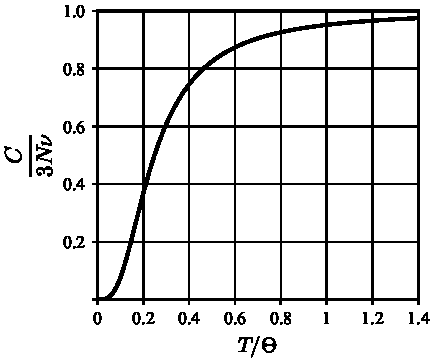
\includegraphics[width=7cm]{fig8.pdf}\\[0.3em]{\small 图 8}\end{minipage}\par\nopagebreak

公式(66.6)—(66.8)就是所求的固体各热力学量的内插公式(P. Debye, 1912).

很容易看到：在两种极限情形下这些公式确实给出了正确的结果.在 $T\ll\Theta$(低温)时德拜函数的宗量 $\dfrac{\Theta}{T}$ 很大.在一级近似下，在德拜函数 D(x) 的定义(66.5)中可以把积分上限 x 用 $\infty$ 代替；所得到的定积分等于 $\dfrac{\pi^4}{15}$，因此\footnote{用积分 $\int_0^\infty-\int_x^\infty$ 代替 $\int_0^x$，在第二个积分的被积式中把 $(\mathrm{e}^x-1)^{-1}$ 按 $\mathrm{e}^{-x}$ 的幂次展开并逐项进行积分，我们求出：当 $x\gg1$ 时，
\begin{equation*}
  D(x)=\frac{\pi^4}{5x^3}-3\mathrm{e}^{-x}\left[1+O\left(\frac{1}{x}\right)\right].
\end{equation*}
因此，在正文中所引用的值，除了未考虑指数小的项以外，是正确的.}
\begin{equation*}
  D(x)\approx\frac{\pi^4}{5x^3}\qquad(x\gg1).
\end{equation*}
把它代入(66.8)，我们得到：
\begin{equation}
  C=\frac{12N\nu\pi^4}{5}\left(\frac{T}{\Theta}\right)^3,
\end{equation}
这同(64.9)是一致的.而在高温($T\gg\Theta$)时德拜函数的宗量很小；当 $x\ll1$ 时，在一级近似下 $D(x)\approx1$\footnote{当 $x\ll1$ 时，把被积式按 $x$ 的幂次直接展开并逐项积分，就得出
\begin{equation*}
  D(x)=1-\frac{3}{8}x+\frac{1}{20}x^2-\cdots.
\end{equation*}}，因而从(66.8)我们有：$C=3N\nu$，又同以前所得的结果(65.5)完全一致\footnote{在高温下，热容精确到展开的下一项为
\begin{equation*}
  C=3N\nu\left[1-\frac{1}{20}\left(\frac{\Theta}{T}\right)^2\right].
\end{equation*}}.

值得指出：函数 $D(x)$ 的实际变化进程表明：热容在两种极限情形下的定律能够适用的判据是 T 和 $\dfrac{\Theta}{4}$ 的相对大小：当 $T\gg\dfrac{\Theta}{4}$ 时热容可以认为是常数，而 $T\ll\dfrac{\Theta}{4}$ 时热容与 $T^3$ 成正比\footnote{举例来说，一些物质从热容数据所得到的 $\Theta$ 值为：Pb 90K, Ag 210K, Al 400K, KBr 180K, NaCl 280K；特别大的是金刚石的 $\Theta$：大约 2000K.}.

根据德拜公式，热容是比值 $\dfrac{\Theta}{T}$ 的某个普适函数.换句话说，根据这个公式处于所谓“对应态”即具有相同的 $\dfrac{\Theta}{T}$ 中的不同物体的热容应该是相同的.

德拜公式只对一些具有简单晶格的固体包括大多数元素和一些简单化合物如卤素盐类固体，才(在对内插公式所能要求的精确程度内)很好地表达了热容随温度变化的进程.对于结构很复杂的物体，实际上它是不适用的；这是很自然的，因为这些物体的振动谱非常复杂.

\section{固体的热膨胀}

在自由能(64.6)中，正比于 $T^4$ 的项在低温下可以认为是附加到 $F_0=N\varepsilon_0\left(\dfrac{V}{N}\right)$ 上的一个很小的增量.从另一方面来看，对自由能的小的修正项(在给定的 V 和 T 下)等于(在给定的 P 和 T 下)对热力学势 $\Phi$ 的小修正项(见(15.12)).因此我们可以立刻写出：
\begin{equation}
  \Phi=\Phi_0(P)-\frac{\pi^2T^4V_0(P)}{30(\hbar\bar{u})^3}.
\end{equation}
式中 $\Phi_0(P)$ 是热力学势中与温度无关的部分，$V_0(P)$ 是体积，借助于
\begin{equation*}
  P=-\frac{\partial F_0}{\partial V}=-N\frac{\mathrm{d}\varepsilon_0}{\mathrm{d}V}
\end{equation*}
表示为压强的函数，而 $\bar{u}=\bar{u}(P)$ 是借助于同一个关系式用压强来表示的平均声速.物体的体积对温度的依赖关系由 $V=\dfrac{\partial\Phi}{\partial P}$ 来决定：
\begin{equation}
  V=V_0(P)-\frac{\pi^2T^4}{30\hbar^3}\frac{\mathrm{d}}{\mathrm{d}P}\left(\frac{V_0}{\bar{u}^3}\right).
\end{equation}
热膨胀系数
\begin{equation}
  \alpha=\frac{1}{V}\left(\frac{\partial V}{\partial T}\right)_P=-\frac{2\pi^2T^3}{15\hbar^3V_0}\frac{\mathrm{d}}{\mathrm{d}P}\left(\frac{V_0}{\bar{u}^3}\right).
\end{equation}
我们看到：在低温下 $\alpha$ 与温度的三次方成正比.虽然如此，但是这个事实早就可以从能斯特定理(§23)和热容的 $T^3$ 定律看出来了.

类似地，在高温下我们把(65.6)中的第二项和第三项看作是对第一项的小修正项(为了使物体是固态的，在任何情形下都应该有 $T\ll\varepsilon_0$)，我们得到：
\begin{equation}
  \Phi=\Phi_0(P)-NcT\ln T+NcT\ln\hbar\bar{\omega}(P).
\end{equation}
由此得出
\begin{equation}
  V=V_0(P)+\frac{NcT}{\bar{\omega}}\frac{\mathrm{d}\bar{\omega}}{\mathrm{d}P}.
\end{equation}
热膨胀系数为
\begin{equation}
  \alpha=\frac{Nc}{V_0\bar{\omega}}\frac{\mathrm{d}\bar{\omega}}{\mathrm{d}P}.
\end{equation}
它是与温度无关的.

随着压强的增加，固体中的原子彼此靠近，而它们振动的振幅(在同一能量值下)减小；换句话说，频率增加.所以 $\dfrac{\mathrm{d}\bar{\omega}}{\mathrm{d}P}>0$，因此 $\alpha>0$，即固体随温度的升高而膨胀.类似的讨论表明：公式(67.3)中的热膨胀系数 $\alpha$ 也是正的.

最后，我们来利用在上一节末尾所指出的对应态定律.热容只是比值 $\dfrac{T}{\Theta}$ 的函数的论断，相当于断言，以热力学势为例，它是如下形式的函数
\begin{equation}
  \Phi=\Phi_0(P)+\Theta f\left(\frac{T}{\Theta}\right).
\end{equation}
同时体积为
\begin{equation*}
  V=V_0(P)+\frac{\mathrm{d}\Theta}{\mathrm{d}P}\left(f-\frac{T}{\Theta}f'\right),
\end{equation*}
而热膨胀系数为
\begin{equation*}
  \alpha=-\frac{T}{V_0\Theta^2}\frac{\mathrm{d}\Theta}{\mathrm{d}P}f''.
\end{equation*}
用类似的方式我们求得焓 $W=\Phi-T\dfrac{\partial\Phi}{\partial T}$ 和热容 $C=\dfrac{\partial W}{\partial T}$：
\begin{equation*}
  C=-\frac{T}{\Theta}f''.
\end{equation*}
比较 C 和 $\alpha$ 的两个表达式，我们得到如下关系式：
\begin{equation}
  \frac{\alpha}{C}=\frac{1}{\Theta V_0(P)}\frac{\mathrm{d}\Theta}{\mathrm{d}P}.
\end{equation}
由此可见，在对应态定律能够适用的范围内，固体热膨胀系数和热容的比值与温度无关(格林艾森定律).

以前我们已经提到过：在固体中热容 $C_p$ 和 $C_v$ 之差是非常小的.在低温范围内，这是由于适用于所有一般物体的能斯特定理的普遍结果.在高温范围内，利用热力学关系式(16.9)，我们有：
\begin{equation*}
  C_p-C_v=-\frac{T\alpha^2V_0^2}{\mathrm{d}V_0/\mathrm{d}P},
\end{equation*}
式中 $\alpha=\alpha(P)$ 是热膨胀系数(67.6).我们看到：$C_p-C_v$ 之差正比于 T；这实质上意味着：它按 $\dfrac{T}{\varepsilon_0}$ 的幂次的展开式是从一次项开始的，但是热容本身的展开式是从零次(常数)项开始的.由此得出结论：固体在高温时也有 $C_p-C_v\ll C$.

\section{高度各向异性的晶体}

在§66末尾已经指出，德拜公式实际上对结构复杂的晶体不适用.这里尤其指“层”型和“链”型的高度各向异性晶体结构.前者可以说是由平行原子层构成，并且在每一层内部原子的相互作用能与相邻层的结合能相比很大，类似地，链型结构由彼此结合相对较弱的平行原子链构成.这些晶体的声波振动谱不是由单个而是由几个数量级不同的德拜温度来表征.只有在温度与德拜温度中的最低一个相比为低时，热容的 $T^3$ 定律才成立；在中间范围内会出现新的极限规律(И.\,М.\,Лифшиц, 1952).

我们首先考虑层型结构.相对于层平面(取作 $xy$ 平面)中的原子振动而言，这种晶格具有最大的硬度；而对于以层为整体的层间相对振动，晶格的硬度很小.这些性质导致三支声波谱有频率依赖于波矢的特征(色散关系)，这里以六方对称晶体为例，它们可以表示为下列公式：
\begin{equation}
\begin{aligned}
  &\omega_1^2=U_1^2\varkappa^2+u_3^2k_z^2,\qquad
   \omega_2^2=U_2^2\varkappa^2+u_3^2k_z^2,\\
  &\omega_3^2=u_3^2\varkappa^2+u_4^2k_z^2,\qquad
   \left(\varkappa^2=k_x^2+k_y^2\right),
\end{aligned}
\end{equation}
此处 $U_1,U_2\gg u_3,u_4$.在这里传播速度 $U_1,U_2$ 属于层平面中的原子振动，$u_3$(在 $\omega_1,\omega_2$ 两支中)属于层间剪切振动，$u_4$ 属于层间距的振动\footnote{关于晶体六方对称的假设并非必不可缺少，这样做只是为了使公式(68.1)更为明确. 速度 $U_1,\cdots,u_4$ 用这种晶体的弹性模量表示如下：
\begin{equation*}
  U_1^2=\frac{1}{\rho}\lambda_{xyxy},\quad U_2^2=\frac{1}{\rho}\lambda_{xxxx},\quad
  u_3^2=\frac{1}{\rho}\lambda_{xzxz},\quad u_4^2=\frac{1}{\rho}\lambda_{zzzz},
\end{equation*}
式中 $\rho$ 是密度.（对于层型晶体，弹性模量 $\lambda_{xzxz}$，$\lambda_{xxzz}$，$\lambda_{zzzz}$ 与模量 $\lambda_{xxxx}$，$\lambda_{xyxy}$ 相比很小，对第七卷§23 的习题 2 中求出的表达式，按前者的幂次展开，可得到这些公式.）正文中所述的振动类型，可以从张量 $\lambda_{iklm}$ 的各个分量的意义予以辨认.}.

然而，对于研究晶体的热性质而言，表达式(68.1)还是不够的.实际上，这些表达式只是函数 $\omega^2(\boldsymbol{k})$ 按波矢幂次展开式的第一项.但是由于这些展开式的二次项的某些系数“反常”的小，下一阶(四次)项也起重要的作用\footnote{确定波的色散关系的方程是 $\omega^2$ 的代数方程（见下节）. 因此，它就是函数 $\omega^2(\boldsymbol{k})$ 按 $k_x,k_y,k_z$ 幂次的正则展开. 考虑到这些函数的偶性（参看§69），展开式仅含偶次项.}.为阐明它们的形式，我们注意到，完全忽略层间耦合时，波的色散关系形为
\begin{equation}
  \omega_1^2=U_1^2\varkappa^2,\qquad
  \omega_2^2=U_2^2\varkappa^2,\qquad
  \omega_3^2=\gamma^2\varkappa^4.
\end{equation}
频率 $\omega_1$ 和 $\omega_2$ 相应于层平面内的纵振动，而频率 $\omega_3$ 相应于横振动，这种情况下是看作自由弹性薄板的片层的弯曲波(参看第七卷§25).所以，略去四次方项中与层间耦合有关的小项，我们最后把波的色散关系写成
\begin{equation}
  \omega_{1,2}^2=U_{1,2}^2\varkappa^2+u_3^2k_z^2,\qquad
  \omega_3^2=u_3^2\varkappa^2+u_4^2k_z^2+\gamma^2\varkappa^4
\end{equation}
我们将认为 $U_1\sim U_2$，$u_3\sim u_4$，并用记号 $\eta\sim\dfrac{u}{U}$ 记小比值，以表征层间耦合能与同层原子间耦合能相比的相对大小.我们也引进像 $\Theta=\hbar\omega_m$ 一样的德拜温度(更确切地说，是德拜温度中最大的)，式中 $\omega_m\sim\dfrac{U}{a}$ 是“硬”振动的极限频率(a 是晶格常数)；“软”振动的极限频率与 $\omega_m$ 相比很小，差一比例 $\eta$.最后，自然可以认为，弯曲波的极限频率与 $\omega_m$ 同数量级或稍小；设它 $\sim\omega_m$\footnote{换言之，我们假设 $\gamma\sim\omega_m a^2\sim Ua$. 应该着重指出，与层的“横向刚度”有关的系数 $\gamma$ 并非可以只用一些弹性模量 $\lambda_{iklm}$ 表达.}.在这些情形下，我们阐明在 $T\ll\Theta$ 下晶体热容的温度依赖关系的特征\footnote{高温 $T\gg\Theta$ 构成经典区域，其中热容 $C=$ 常数.}.

考虑声学振动的贡献，物体的自由能取决于公式
\begin{equation}
  F=N\varepsilon_0+T\sum_{\alpha=1}^{3}\int\ln\left(1-\mathrm{e}^{-\hbar\omega_\alpha/T}\right)\frac{V\,\mathrm{d}k_x\,\mathrm{d}k_y\,\mathrm{d}k_z}{(2\pi)^3},
\end{equation}
式中求和对波谱的三个支进行，而积分遍及波矢变化的所有区域\footnote{也就是一个倒格子胞；参看下面的公式(71.7).}.

如果 $T\gg\eta\Theta$，则可以忽略层间耦合，并相应地利用谱(68.2).对自由能的主要贡献来自“弯曲”支 $\omega_3$.由于 $T\ll\Theta$ 时收敛很快，关于 $\mathrm{d}k_x\,\mathrm{d}k_y$ 的积分可以扩展为从 $-\infty$ 到 $\infty$.用对 $2\pi\varkappa\,\mathrm{d}\varkappa$ 的积分取代它，经此显而易见的代换，求得
\begin{equation*}
  \int_0^{\infty}\ln\left(1-\mathrm{e}^{-\hbar\gamma\varkappa^2/T}\right)2\pi\varkappa\,\mathrm{d}\varkappa
  =\frac{\pi T}{\hbar\gamma}\int_0^{\infty}\ln\left(1-\mathrm{e}^{-x}\right)\mathrm{d}x.
\end{equation*}
对 $\mathrm{d}k_z$ 的积分(区域取 $|k_z|\leqslant k_{z\max}\sim\dfrac{1}{a}$)给出与温度无关的因子 $\sim\dfrac{1}{a}$.结果求得自由能的温度部分正比于 $T^2$，相应地对于热容有
\begin{equation}
  C\propto T\qquad\text{当}\ \eta\Theta\ll T\ll\Theta\ \text{时}.
\end{equation}
当 $T\ll\eta\Theta$ 时，在积分(68.4)中必须写出 $\omega_\alpha(\boldsymbol{k})$ 的完全表达式(68.3)，而对 k 的各个分量的积分可以扩展为从 $-\infty$ 到 $\infty$.这样得到的自由能的温度关系足够复杂，但是仍然可以分出两种极限情形.如果 $T\gg\eta^2\Theta$，则主要的贡献还是来自 $\omega_3$ 一支，且可略去它的 $\varkappa^2$ 项，写成
\begin{equation*}
  \omega_3^2=u_4^2k_z^2+\gamma^2\varkappa^4.
\end{equation*}
实际上，$\varkappa\,\mathrm{d}\varkappa$ 的积分中起主要作用的是如下的值：$\hbar\gamma\varkappa^2\sim T$，这时 $\hbar u\varkappa\sim\hbar u\left(T/\hbar\gamma\right)^{1/2}\sim T\left(\eta^2\Theta/T\right)^{1/2}\ll T$.现在我们求得
\begin{equation*}
  \int_{-\infty}^{\infty}\int_0^{\infty}\ln\left[1-\exp\left(-\frac{\hbar}{T}\sqrt{u_4^2k_z^2+\gamma^2\varkappa^4}\right)\right]2\pi\varkappa\,\mathrm{d}\varkappa\,\mathrm{d}k_z
  =\text{常数}\cdot\frac{T^2}{u_4\gamma},
\end{equation*}
结果，对于热容有
\begin{equation}
  C\propto T^2\qquad\text{当}\ \eta^2\Theta\ll T\ll\eta\Theta\ \text{时}.
\end{equation}
最后，在 $T\ll\eta^2\Theta$ 时用同样的方法可以证明在(68.3)中可略 $\varkappa^4$ 项，于是我们回到 $\omega$ 线性依赖于 k 的声波谱(68.1)，对于热容得到德拜定律
\begin{equation}
  C\propto T^3\qquad\text{当}\ T\ll\eta^2\Theta\ \text{时}.
\end{equation}

用类似的方法可以考虑链型结构的晶体(选取链方向为 z 轴).在这种情形下，声波谱三个分支的色散关系有下列形式
\begin{equation}
  \omega_{1,2}^2=u_{1,2}^2\varkappa^2+u_3^2k_z^2+\gamma^2k_z^4,\qquad
  \omega_3^2=u_3^2\varkappa^2+U_4^2k_z^2,
\end{equation}
而且现在 $u_1,u_2,u_3\ll U_4$\footnote{为明确起见，这里再次假设六方对称——这一次是指链方向. 速度 $u_1,\cdots,U_4$ 用本节第一个脚注中提到的同样的公式由弹性模量表达，但是现在模量 $\lambda_{xxxx}$，$\lambda_{xyxy}$，$\lambda_{xzxz}$，$\lambda_{yzyz}$ 与 $\lambda_{zzzz}$ 相比为小.}.略去链间相互作用，关系(68.8)归于
\begin{equation*}
  \omega_{1,2}^2=\gamma^2k_z^4,\qquad
  \omega_3^2=U_4^2k_z^2;
\end{equation*}
谱支 $\omega_3$ 对应于链中原子的纵振动，$\omega_1$ 和 $\omega_2$ 对应于把链看成弹性弦时的弯曲波.设 $u_1\sim u_2\sim u_3$ 并且仍旧引进小参量 $\eta\sim\dfrac{u}{U}$ 和德拜温度，可以得出下列热容与温度依赖关系的极限规律：
\begin{equation}
\left.\begin{aligned}
  \text{当}\ \eta\Theta\ll T\ll\Theta\ \text{时},\qquad &C\propto T^{1/2},\\
  \text{当}\ \eta^2\Theta\ll T\ll\eta\Theta\ \text{时},\qquad &C\propto T^{3/2},\\
  \text{当}\ T\ll\eta^2\Theta\ \text{时},\qquad &C\propto T^3.
\end{aligned}\right\}
\end{equation}

\section{晶格的振动}

在上节中我们把固体中原子的热运动考虑为晶格的简正微振动的集合.现在我们来更仔细地研究这些振动的力学性质.

在晶体的每个单胞中一般来讲有若干个原子.因此要指定一个原子必须给出它所处的单胞以及这个原子在该胞中的编号.单胞的位置可以用单胞的任意一个特定顶点的径矢 $\boldsymbol{r}_{\boldsymbol{n}}$ 来确定.这些径矢的取值为
\begin{equation}
  \boldsymbol{r}_{\boldsymbol{n}}=n_1\boldsymbol{a}_1+n_2\boldsymbol{a}_2+n_3\boldsymbol{a}_3,
\end{equation}
式中 $n_1,n_2,n_3$ 是整数，而 $\boldsymbol{a}_1,\boldsymbol{a}_2,\boldsymbol{a}_3$ 是基格矢(即单胞的边长).

我们用 $\boldsymbol{u}_s$ 表示振动的原子位移，式中角标 s 表示原子在胞中的编号($s=1,2,\cdots,\nu$；$\nu$ 是胞中的原子数目).作为在平衡位置(格点)附近作微振动的粒子力学系统，晶格的拉格朗日函数具有形式
\begin{equation}
  L=\frac{1}{2}\sum_{\boldsymbol{n},s}m_s\dot{\boldsymbol{u}}_s^2(\boldsymbol{n})
  -\frac{1}{2}\sum_{\boldsymbol{n}\boldsymbol{n}'}\Lambda_{ik}^{ss'}\left(\boldsymbol{n}-\boldsymbol{n}'\right)
  u_{si}(\boldsymbol{n})u_{s'k}(\boldsymbol{n}'),
\end{equation}
式中矢量 $\boldsymbol{n}=(n_1,n_2,n_3)$；$m_s$ 是原子的质量，而 i,\,k 是矢量指标，取值 $x,y,z$(而且依惯例二次重复指标意味着求和).系数 $\Lambda$ 仅仅依赖于差 $\boldsymbol{n}-\boldsymbol{n}'$，因为原子间相互作用力仅仅依赖于晶格单胞的相对位置，而与它们在空间的绝对位置无关.这些系数具有对称性
\begin{equation}
  \Lambda_{ik}^{ss'}(\boldsymbol{n})=\Lambda_{ki}^{s's}(-\boldsymbol{n}),
\end{equation}
这从函数(69.2)的形式显而易见.

从拉格朗日函数(69.2)可得运动方程
\begin{equation}
  m_s\ddot{u}_{si}(\boldsymbol{n})
  =-\sum_{\boldsymbol{n}'s'}\Lambda_{ik}^{ss'}\left(\boldsymbol{n}-\boldsymbol{n}'\right)u_{s'k}\left(\boldsymbol{n}'\right).
\end{equation}
应该指出，各系数 $\Lambda$ 以特定的关系互相联系，体现如下事实：晶格作为整体作平移或者转动时不会对原子产生任何的作用力.在平移时所有的 $\boldsymbol{u}_s(\boldsymbol{n})=$ 常数，因此应有
\begin{equation}
  \sum_{\boldsymbol{n}}\Lambda_{ik}^{ss'}(\boldsymbol{n})=0.
\end{equation}
在这里我们不写出从相对转动不变性得出的关系.

我们求方程(69.4)的单色平面波形式的解
\begin{equation}
  \boldsymbol{u}_s(\boldsymbol{n})
  =\boldsymbol{e}_s(\boldsymbol{k})\exp\left[\mathrm{i}\left(\boldsymbol{k}\cdot\boldsymbol{r}_{\boldsymbol{n}}-\omega t\right)\right].
\end{equation}
(复)振幅 $\boldsymbol{e}_s$ 仅依赖于角标 s，即仅对同一胞内的不同原子有所不同，而不管不同胞中的等效原子.矢量 $\boldsymbol{e}_s$ 既决定振幅的大小，也决定它们偏振的方向.

把(69.6)代入(69.4)，我们得到
\begin{equation*}
  \omega^2m_se_{si}\exp\left(\mathrm{i}\boldsymbol{k}\cdot\boldsymbol{r}_{\boldsymbol{n}}\right)
  =\sum_{\boldsymbol{n}'s'}\Lambda_{ik}^{ss'}\left(\boldsymbol{n}-\boldsymbol{n}'\right)
  e_{s'k}\exp\left(\mathrm{i}\boldsymbol{k}\cdot\boldsymbol{r}_{\boldsymbol{n}'}\right).
\end{equation*}
等式的两边除以 $\exp\left(\mathrm{i}\boldsymbol{k}\cdot\boldsymbol{r}_{\boldsymbol{n}}\right)$ 并用对 $\boldsymbol{n}'-\boldsymbol{n}$ 的求和取代对 $\boldsymbol{n}'$ 的求和，得出
\begin{equation}
  \sum_{s'}\Lambda_{ik}^{ss'}(\boldsymbol{k})e_{s'k}-\omega^2m_se_{si}=0,
\end{equation}
式中引入记号
\begin{equation}
  \Lambda_{ik}^{ss'}(\boldsymbol{k})
  =\sum_{\boldsymbol{n}}\Lambda_{ik}^{ss'}(\boldsymbol{n})\exp\left(-\mathrm{i}\boldsymbol{k}\cdot\boldsymbol{r}_{\boldsymbol{n}}\right).
\end{equation}
振幅的线性齐次代数方程组(69.7)有非零解，必须满足如下相容性条件
\begin{equation}
  \det\left|\Lambda_{ik}^{ss'}(\boldsymbol{k})-\omega^2m_s\delta_{ik}\delta_{ss'}\right|=0.
\end{equation}
指标 i,\,k 各取 3 值，而指标 $s,s'$ 各取 $\nu$ 值，因此行列式的阶数等于 $3\nu$，(69.9)是关于 $\omega^2$ 的 $3\nu$ 次代数方程.

这个方程 $3\nu$ 个解的每一个都决定频率 $\omega$ 依赖于波矢 $\boldsymbol{k}$ 的函数关系；这种关系称为波的色散关系，而决定这种关系的方程(69.6)称为色散方程.因此，对于波矢的每一个给定值，在一般情况下，频率可以有 $3\nu$ 个不同的值.可以说频率是波矢的多值函数，有 $3\nu$ 个支，$\omega=\omega_\alpha(\boldsymbol{k})$，这里指标 $\alpha$ 标记函数支.

从定义(69.8)和等式(69.3)得出
\begin{equation}
  \Lambda_{ik}^{ss'}(\boldsymbol{k})
  =\Lambda_{ik}^{s's}(-\boldsymbol{k})
  =\left[\Lambda_{ik}^{s's}(\boldsymbol{k})\right]^{*}.
\end{equation}
换句话说，$\Lambda_{ik}^{ss'}(\boldsymbol{k})$ 各量组成厄米矩阵，从数学观点看来，解方程(69.7)的问题就是求解该矩阵的本征值及相应“本征矢量”的问题.根据厄米矩阵的已知性质，相应于不同本征值的本征矢量相互正交.现在这意味着
\begin{equation}
  \sum_{s=1}^{\nu}m_s\boldsymbol{u}_s^{(\alpha)}\boldsymbol{u}_s^{(\alpha')*}=0
  \qquad\text{当}\ \alpha\neq\alpha',
\end{equation}
位移矢量的角标 $(\alpha)$ 表示它所属的振动谱支\footnote{在关系式(69.11)中出现了“权重”因子 $m_s$. 这是因为 $\omega_\alpha^2$ 并非矩阵 $\Lambda_{ik}^{ss'}(\boldsymbol{k})$ 而是矩阵 $\Lambda_{ik}^{ss'}/\sqrt{m_s m_{s'}}$ 的本征值，并且相应的本征矢量是 $\sqrt{m_s}\,\boldsymbol{u}_s^{(\alpha)}$.}.等式(69.11)表示不同谱支偏振的正交性.

因为力学运动方程关于时间变号的对称性，如果某种波(69.6)的传播是可能的，则同样的波也可以在相反方向传播.但是这种方向的改变等价于 $\boldsymbol{k}$ 的符号改变.因此，$\omega(\boldsymbol{k})$ 应该是偶函数
\begin{equation}
  \omega(-\boldsymbol{k})=\omega(\boldsymbol{k}).
\end{equation}

晶格振动的波矢具有如下重要性质.波矢只通过指数因子 $\exp\left(\mathrm{i}\boldsymbol{k}\cdot\boldsymbol{r}_{\boldsymbol{n}}\right)$ 出现在(69.11)中.但是该因子在如下代换下完全不变：
\begin{equation}
  \boldsymbol{k}\to\boldsymbol{k}+\boldsymbol{b},\qquad
  \boldsymbol{b}=p_1\boldsymbol{b}_1+p_2\boldsymbol{b}_2+p_3\boldsymbol{b}_3,
\end{equation}
式中 $\boldsymbol{b}$ 是任意的倒格矢($\boldsymbol{b}_1,\boldsymbol{b}_2,\boldsymbol{b}_3$ 是它的基本周期；$p_1,p_2,p_3$ 是整数)\footnote{这里用到的一些概念，在下面§133会详细考虑.}.换句话说，晶格振动的波矢在物理上不是单值的：相差 $\boldsymbol{b}$ 的所有 $\boldsymbol{k}$ 值在物理上都是等价的.函数 $\omega(\boldsymbol{k})$ 在倒格子中是周期的：
\begin{equation*}
  \omega(\boldsymbol{k}+\boldsymbol{b})=\omega(\boldsymbol{k}),
\end{equation*}
因而在 $\omega(\boldsymbol{k})$ 的每一支中只要考虑波矢 $\boldsymbol{k}$ 的某个有限范围即一个倒格子胞.例如，如果选取坐标轴(在一般情况下是斜交的)沿倒格子的三个基本周期，可以只考虑如下区域
\begin{equation}
  -\frac{1}{2}b_i<k_i\leqslant\frac{1}{2}b_i.
\end{equation}
当 $\boldsymbol{k}$ 取这个区的值时，每个谱支的频率 $\omega(\boldsymbol{k})$ 取占有某个有限宽波段(或称为区)的值.当然不同区可能部分交叠.

用几何的术语来说，函数关系 $\omega=\omega(\boldsymbol{k})$ 表示为四维超曲面，它的各个叶对应于函数的不同支.这些叶可能并不是完全分开的，即可能相交.这些相交的可能类型相当依赖于晶格的具体对称性.研究这个问题需要应用群论方法，这将在以后§136中讨论.

在 $3\nu$ 支振动的波谱中，必定有一些波长(与晶格常数相比大的)很大，对应于晶体中通常的弹性波(即声波).从弹性理论(参看第七卷§23)知，当成连续介质的晶体可以传播具有不同色散关系的三种波，并且对于所有这三种类型，$\omega$ 是矢量 $\boldsymbol{k}$ 的分量的一次齐次函数，且在 $\boldsymbol{k}=0$ 时变为 0.因此，在函数 $\omega(\boldsymbol{k})$ 的 $3\nu$ 支中应该有三支，在 $\boldsymbol{k}$ 很小时其色散关系形为
\begin{equation}
  \omega=kf\left(\frac{\boldsymbol{k}}{k}\right)
\end{equation}
这三型波称为声学波；它们的特征是：(在 $\boldsymbol{k}$ 很小时)晶格像连续介质一样整体地振动.在 $\boldsymbol{k}\to0$ 的极限情形下，这些振动变为整个晶格的简单平移.

在每胞含有多于一个原子的复杂晶格中，还存在 $3(\nu-1)$ 个类型的波.这些波谱支在 $\boldsymbol{k}=0$ 时频率并不变为 0，当 $\boldsymbol{k}\to0$ 时趋于常数极限.晶格的这些振动称为光学振动.在这种情形下，同一单胞中的原子彼此相对运动，并且在 $\boldsymbol{k}=0$ 的极限情形下，胞的重心保持不动\footnote{后一结论可以从运动方程(69.7)，(69.8)直接正式导出. 在 $\boldsymbol{k}=0$ 时，方程形为
\begin{equation*}
  \sum_{\boldsymbol{n}s'}\Lambda_{ik}^{ss'}(\boldsymbol{n})\,e_{s'k}=m_s\omega^2 e_{si}.
\end{equation*}
方程两边对 $s$ 求和，因为(69.5)而左边得到 0；所以为使方程在 $\boldsymbol{k}=0$ 时仍然对，应该也有 $\sum_s m_s e_{si}=0$.}.

所有 $3(\nu-1)$ 个光学振动的极限频率($\boldsymbol{k}=0$ 时的频率)不一定都各不相同.在具有一定对称的晶体中，某些光学谱支的极限频率可能重合，或者说是简并的(关于这一点参看§136).

具有非简并极限频率的函数 $\omega(\boldsymbol{k})$ 可以在 $\boldsymbol{k}=0$ 的附近展开为矢量 $\boldsymbol{k}$ 的分量的幂级数.由于 $\omega(\boldsymbol{k})$ 是偶函数，这种展开式只含 $k_i$ 的偶次幂，因此它的前几项形为
\begin{equation}
  \omega=\omega_0+\frac{1}{2}\gamma_{ik}k_ik_k,
\end{equation}
式中 $\omega_0$ 是极限频率，$\gamma_{ik}$ 是一些常数.

然而，如果有几支的极限频率相同，则这些支中的频率函数 $\omega(\boldsymbol{k})$ 完全不能按 $\boldsymbol{k}$ 的幂次展开，因为 $\boldsymbol{k}=0$ 的点是它们的奇点(分支点).这时只能够断言：在 $\boldsymbol{k}=0$ 的附近差 $\omega-\omega_0$ 是 $\boldsymbol{k}$ 的分量的一次或二次齐次函数(依晶体的对称而定).

我们再次提醒：上述的一切讨论都是在所谓的“简谐近似”之下，这时势能只考虑原子位移的二次项.只有在这种近似下，各种不同的单色波(69.6)才彼此没有相互作用，而自由地在晶格中传播.在考虑后面的“非简谐”项后，就会出现这些波的相互散射和各种衰减过程.相互作用也可能导致形成波的“束缚态”(声子，见下)，这是简谐近似下所没有的波谱新支.

此外，我们假定了晶格具有理想的周期性.必须注意：只要在晶体中有各种同位素的原子以无序方式分布着(即使不考虑可能的“杂质”以及晶格的其它缺陷)，理想的周期性在某种程度上也是被破坏了的.但是，如果这些同位素的原子量相对差很小，或者一种同位素比其余的多很多，则这种破坏比较不重要.在这些情形下，一级近似下所述的图像仍然有效，但是在更高级的近似下，就会产生波受晶格不均匀性散射的各种类型的过程\footnote{晶格缺陷的存在也引起振动谱的某些变化. 出现一些新频率（对应于在缺陷附近的“局域化”振动）. 这些问题的研究见：Лифшиц И М, Косевич А М. Динамика кристаллической решетки с дефектами. Rep.~Progr.~Phys., 1966, 29: 217. Перевод в книге: Лифшиц И М. Избранные труды. Физика реальных кристаллов и неупорядоченных систем. Наука, 1987, статья 14.}.

\section{振动数的态密度}

波矢分量值处在区间 $\mathrm{d}^3\boldsymbol{k}\equiv\mathrm{d}k_x\,\mathrm{d}k_y\,\mathrm{d}k_z$ 内的振动数，对晶体单位体积而言等于 $\dfrac{\mathrm{d}^3k}{(2\pi)^3}$.振动按频率的分布函数 $g(\omega)$ 是具体晶格的振动谱特征，由它给出，频率位于 $\omega$ 到 $\omega+\mathrm{d}\omega$ 之间的振动数为 $g(\omega)\mathrm{d}\omega$.当然，对于不同的谱支这个数是不同的，但是为了简化记号，本节略去函数 $\omega(\boldsymbol{k})$ 和 $g(\omega)$ 的相应角标 $\alpha$.

数 $g(\omega)\mathrm{d}\omega$ 等于 k 空间中包围在两个无限接近的等频面 $\omega(\boldsymbol{k})=$ 常数之间的体积除以 $(2\pi)^3$.函数 $\omega(\boldsymbol{k})$ 在 k 空间每一点的梯度，指向过该点的等频面的法线.因此，从表达式 $\mathrm{d}\omega=\mathrm{d}\boldsymbol{k}\cdot\nabla_{\boldsymbol{k}}\omega(\boldsymbol{k})$ 可明显看出，这样的两个无限接近表面的间距(用它们之间的法线一段量度)是 $\dfrac{\mathrm{d}\omega}{|\nabla_{\boldsymbol{k}}\omega|}$.把这个量乘以等频面的面元 $\mathrm{d}f_{\boldsymbol{k}}$ 并对整个表面积分(在一个倒格子胞的范围内)，我们得到待求的 k 空间体积部分，把它除以 $(2\pi)^3$，即为频率分布密度：
\begin{equation}
  g(\omega)=\frac{1}{(2\pi)^3}\int\frac{\mathrm{d}f_{\boldsymbol{k}}}{\left|\nabla_{\boldsymbol{k}}\omega(\boldsymbol{k})\right|}.
\end{equation}
在每区(某支 $\omega(\boldsymbol{k})$ 在 k 的一个倒格子胞内所取的值域)中，函数 $\omega(\boldsymbol{k})$ 应该至少有一个极小和一个极大.因而，由此得出，该函数也应该具有鞍点\footnote{可以证明（但不在这里给出），至少应该存在 6 个鞍点，两类各三个，对应于公式(70.8)（参看下面）中的 $+$ 号和 $-$ 号.}.所有这些稳恒点的存在导致频率分布函数 $g(\omega)$ 的一定特征(L.~van Hove, 1953).

在位于某个 $\boldsymbol{k}=\boldsymbol{k}_0$ 的极值点附近，记 $\omega_0=\omega(\boldsymbol{k}_0)$，差值 $\omega(\boldsymbol{k})-\omega_0$ 具有形式
\begin{equation*}
  \omega-\omega_0=\frac{1}{2}\gamma_{ik}\left(k_i-k_{0i}\right)\left(k_k-k_{0k}\right).
\end{equation*}
取 k 空间的坐标轴沿该二次型的主轴，我们把它写成
\begin{equation}
  \omega-\omega_0=\frac{1}{2}\left[\gamma_1(k_x-k_{0x})^2+\gamma_2(k_y-k_{0y})^2+\gamma_3(k_z-k_{0z})^2\right],
\end{equation}
式中 $\gamma_1,\gamma_2,\gamma_3$ 是对称张量 $\gamma_{ik}$ 的主值.

我们首先考虑函数 $\omega(\boldsymbol{k})$ 的一个极小点或极大点.于是 $\gamma_1,\gamma_2,\gamma_3$ 有相同的符号.根据 $\varkappa_x=\sqrt{|\gamma_1|}\left(k_x-k_{0x}\right),\cdots$，引入新变量 $\varkappa_x,\varkappa_y,\varkappa_z$ 代换 $k_x,k_y,k_z$，我们写出
\begin{equation}
  \omega-\omega_0=\pm\frac{1}{2}\left(\varkappa_x^2+\varkappa_y^2+\varkappa_z^2\right)=\pm\frac{1}{2}\varkappa^2.
\end{equation}
这时在 $\varkappa$ 空间中的等频面是球面.在(70.1)中变换到 $\varkappa$ 空间中的积分，有
\begin{equation}
  g(\omega)=\frac{1}{(2\pi)^3\sqrt{\gamma}}\int\frac{\mathrm{d}f_{\varkappa}}{\left|\nabla_{\varkappa}\omega(\varkappa)\right|},\qquad
  \gamma=\left|\gamma_1\gamma_2\gamma_3\right|,
\end{equation}
球面元为：$\mathrm{d}f_{\varkappa}=\varkappa^2\,\mathrm{d}O_{\varkappa}$，式中 $\mathrm{d}O_{\varkappa}$ 是立体角元.函数(70.3)的梯度为：$\nabla_{\varkappa}\omega(\varkappa)=\pm\varkappa$.所以(70.4)中的积分等于 $4\pi\varkappa$；根据(70.3)用 $\omega-\omega_0$ 表示 $\varkappa$，最后得
\begin{equation}
  g(\omega)=\frac{1}{\pi^2\sqrt{2\gamma}}\sqrt{\left|\omega-\omega_0\right|}.
\end{equation}
因此，振动数密度具有平方根奇异性；微商 $\dfrac{\mathrm{d}g}{\mathrm{d}\omega}$ 在 $\omega\to\omega_0$ 时变为无穷大.

但是，应该注意到，在一般情形下(如果值 $\omega=\omega_0$ 位于频率变化带的内部而非正好边缘上)，值 $\omega$ 接近 $\omega_0$ 的等频面(除了包含 $\boldsymbol{k}=\boldsymbol{k}_0$ 点周围的椭球面以外)还可能包含位于 k 空间中单胞其它部分的其它叶.因此在一般情况下表达式(70.5)只给出振动数密度的“奇异”部分，因而更正确地应该对 $\omega=\omega_0$ 点的一侧(对极大为 $\omega<\omega_0$，而对极小为 $\omega>\omega_0$)写
\begin{equation}
  g(\omega)=g(\omega_0)+\frac{\sqrt{\left|\omega-\omega_0\right|}}{\pi^2\sqrt{2\gamma}},
\end{equation}
而对另一侧，写 $g(\omega)=g(\omega_0)$.

我们也注意到，公式(70.5)自然并不属于声学振动区的下缘($\omega=0$)的邻域，那里色散关系形为(69.15).容易看出，在这种情形下
\begin{equation}
  g(\omega)=\text{常数}\cdot\omega^2.
\end{equation}
现在我们考虑鞍点的邻域.在这种情况下(70.2)中 $\gamma_1,\gamma_2,\gamma_3$ 的值，两正，一负，或者一正两负.代替(70.3)现在有
\begin{equation}
  \omega-\omega_0=\pm\frac{1}{2}\left(\varkappa_x^2+\varkappa_y^2-\varkappa_z^2\right).
\end{equation}
为明确起见，取该式中上号.于是，在 $\omega<\omega_0$ 时等频面是双叶双曲面，而在 $\omega>\omega_0$ 时是单叶双曲面；$\omega=\omega_0$ 的分界面是双锥面(图9).

\par\nopagebreak\noindent\begin{minipage}{\linewidth}\centering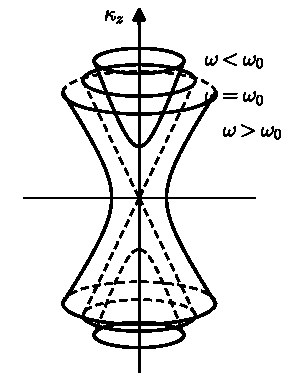
\includegraphics[width=6cm]{fig9.pdf}\\[0.3em]{\small 图 9}\end{minipage}\par\nopagebreak

在(70.4)中的积分现在很容易计算，如果用 $\varkappa$ 空间的圆柱坐标系：$\varkappa_{\perp},\varkappa_z,\varphi$，这里 $\varkappa_{\perp}=\sqrt{\varkappa_x^2+\varkappa_y^2}$，而 $\varphi$ 是 $\varkappa_x,\varkappa_y$ 平面中的极角.梯度的绝对值为：$\left|\nabla_{\varkappa}\omega\right|=\varkappa$.当 $\omega<\omega_0$ 时，积分在双曲面的两腔中进行：
\begin{equation*}
\begin{gathered}
  \mathrm{d}f_{\varkappa}=\frac{2\pi\varkappa_{\perp}\varkappa}{\left|\varkappa_z\right|}\,\mathrm{d}\varkappa_{\perp},\\
  g(\omega)=\frac{1}{(2\pi)^3\sqrt{\gamma}}\cdot2\int_0^{K}\frac{2\pi\varkappa_{\perp}\,\mathrm{d}\varkappa_{\perp}}{\sqrt{\varkappa_{\perp}^2+2\left(\omega_0-\omega\right)}}\,;
\end{gathered}
\end{equation*}
作为上限 K(其值不影响最终奇异性的形式)可以取任何比 $\sqrt{\omega_0-\omega}$ 为大的 $\varkappa$ 值，但是同时又如此之小，以至于表达式(70.8)仍有等频面的形式.结果求得
\begin{equation*}
  g(\omega)=\frac{1}{2\pi^2\sqrt{\gamma}}\left[K-\sqrt{2\left(\omega_0-\omega\right)}\right].
\end{equation*}
在 $\omega>\omega_0$ 的情形下，用类似的方法可以求得
\begin{equation*}
  g(\omega)=\frac{2}{(2\pi)^3\sqrt{\gamma}}\int_{\varkappa_{\perp\min}}^{K}\frac{2\pi\varkappa_{\perp}\,\mathrm{d}\varkappa_{\perp}}{\sqrt{\varkappa_{\perp}^2-2\left(\omega-\omega_0\right)}}=\frac{K}{2\pi^2\sqrt{\gamma}},
\end{equation*}
式中 $\varkappa_{\perp\min}^2=2\left(\omega-\omega_0\right)$.因此，鞍点邻域的振动数密度具有形式
\begin{equation}
  g(\omega)=\left\{
  \begin{array}{ll}
    g(\omega_0)-\dfrac{\sqrt{\left|\omega_0-\omega\right|}}{\pi^2\sqrt{2\gamma}}\qquad & \text{当}\ \omega<\omega_0,\\[1.2em]
    g(\omega_0)\qquad & \text{当}\ \omega>\omega_0.
  \end{array}\right.
\end{equation}
这里 $g(\omega)$ 也具有平方根奇异性.

对于(70.8)中下号的鞍点，结果类似，不过区域 $\omega<\omega_0$ 和 $\omega>\omega_0$ 互换($\omega>\omega_0$ 时有平方根奇异性).

\section{声子}

现在我们转到从量子理论的观点来看晶格的振动是怎样一种图像的问题.

波(69.6)中原子在每一时刻都有确定的位移，在量子理论中取代波而引入所谓“声子”的概念，它们是一些在晶格中传播的具有确定能量和运动方向的“准粒子”.在量子力学中振子的能量是 $\hbar\omega$(这里 $\omega$ 是经典波的频率)的整数倍，所以声子的能量与频率 $\omega$ 的关系为
\begin{equation}
  \varepsilon=\hbar\omega,
\end{equation}
与光量子——光子——的情况相类似.至于波矢 $\boldsymbol{k}$，则它确定声子的所谓“准动量”$\boldsymbol{p}$：
\begin{equation}
  \boldsymbol{p}=\hbar\boldsymbol{k}.
\end{equation}
这个量在许多方面与通常的动量相似.同时，它们之间又有重大差别，源于如下事实：准动量只能精确到可以附加一个形为 $\hbar\boldsymbol{b}$ 的任意常数矢量的程度；所有相差这样一个量的不同的 $\boldsymbol{p}$ 值在物理上是等价的.

声子的速度取决于相应经典波的群速度 $\boldsymbol{v}=\dfrac{\partial\omega}{\partial\boldsymbol{k}}$.这个公式也可以写成
\begin{equation}
  \boldsymbol{v}=\frac{\partial\varepsilon(\boldsymbol{p})}{\partial\boldsymbol{p}},
\end{equation}
与粒子的能量、动量和速度之间通常的关系式完全相似.

在§69，§70中所述的有关晶格经典振动谱的全部特性完全可以转移(适当改变术语)到声子的能谱即它们的能量与准动量的依赖关系上.例如，声子的能谱 $\varepsilon(\boldsymbol{p})$ 有 $3\nu$ 个不同的支，其中包括三个声学支.在§70中考虑的振动数密度现在变成声子的量子态密度.

在量子图像中，无相互作用声子的自由运动对应于在简谐近似下波的自由传播.在更高级的近似下出现声子碰撞的各种过程.这些碰撞形成了声子气体热平衡，即晶格平衡的热运动得以建立的机制.

在所有这些过程中必须遵守能量守恒定律以及准动量守恒定律.但是后者对声子总准动量只要求守恒到可以附加形为 $\hbar\boldsymbol{b}$ 的任何一个矢量的程度，这与准动量本身的非单值性有关.因此，在任何一个声子碰撞过程中，起始准动量($\boldsymbol{p}$)与最后准动量($\boldsymbol{p}'$)应该由如下形式的关系式相联系\footnote{总准动量并不保持为常数而是改变 $\hbar\boldsymbol{b}$ 的过程，称为折返过程.}
\begin{equation}
  \sum\boldsymbol{p}=\sum\boldsymbol{p}'+\hbar\boldsymbol{b}'.
\end{equation}
在晶格中可以同时激发任意个全同声子；换句话说，处于声子的每一个量子态中的声子数可以是任意的(在经典图像中这对应于波的任意强度).这意味着声子气体遵守玻色统计.在这种气体中粒子总数不是给定的，而是取决于平衡条件，因此它的化学势等于零(参看§63).因而每一个量子态(具有准动量 $\boldsymbol{p}$ 和能量 $\varepsilon$)的声子平均数，在热平衡时由普朗克分布函数确定
\begin{equation}
  \bar{n}_{\boldsymbol{p}}=\frac{1}{\mathrm{e}^{\varepsilon(\boldsymbol{p})/T}-1}.
\end{equation}
应当指出，在高温下($T\gg\varepsilon$)，这个表达式变为
\begin{equation}
  \bar{n}_{\boldsymbol{p}}=\frac{T}{\varepsilon(\boldsymbol{p})},
\end{equation}
即在该状态中的声子数与温度成正比.

声子的概念，对于在任何宏观物体的量子能谱理论中起重要作用的更一般概念而言只是特例.宏观物体的任何弱激发态可以看成各个元激发的集合.这些元激发相当于在物体所占体积中运动的某几种准粒子.只要元激发的数目足够小，它们彼此“不相互作用”(即能量直接可加)，因此它们的集合可以看成准粒子的理想气体.我们再一次强调：元激发的概念只是作为物体中原子集体运动的量子力学描述方法，绝不能把它们混同于个别的原子或分子.

在声子的情形下，它们的相互作用对应于(在经典图像中)晶格原子的非简谐振动.但是，正如§64中所指出的，在固体中这些振动事实上总是很小，因此是“几乎简谐的”.所以，在固体中声子的相互作用事实上总是很弱.

最后，我们写出根据固体声子谱确定的固体热力学量的公式.

固体在热力学平衡态中的自由能由公式(64.1)给出.把其中求和变为对一系列连续声子态的积分，有
\begin{equation}
  F=N\varepsilon_0+T\sum_{\alpha=1}^{3\nu}\int\ln\left[1-\exp\left(-\frac{\hbar\omega_\alpha(\boldsymbol{k})}{T}\right)\right]\frac{V\,\mathrm{d}^3k}{(2\pi)^3},
\end{equation}
式中求和对所有的谱支进行，而积分对一个倒格子胞中的 $\boldsymbol{k}$ 值进行\footnote{这个公式已经在§68中用于处理声学谱支对自由能的贡献.}.对各谱支引入状态数密度 $g_\alpha(\omega)$ 并转换为对频率的积分，这个公式也可以写成
\begin{equation}
  F=N\varepsilon_0+TV\sum_{\alpha=1}^{3\nu}\int\ln\left(1-\mathrm{e}^{-\hbar\omega/T}\right)g_\alpha(\omega)\,\mathrm{d}\omega.
\end{equation}

固体的非平衡宏观状态用声子按它们的量子态的某个非平衡态分布来描述，完全类似于对理想气体所作过的那样.物体在这种状态下的熵可以用§55中(对于玻色气体)所得的公式来计算.尤其是，如果每个状态有许多声子，熵等于
\begin{equation*}
  S=\sum_jG_j\ln\frac{\mathrm{e}N_j}{G_j},
\end{equation*}
式中 $N_j$ 是一组 $G_j$ 个邻近状态中的声子数(参看(55.8)).这种情形对应于高温($T\gg\Theta$).把这个公式改写成对应于热振动经典图像的积分形式.处于波矢值区间 $\mathrm{d}^3k$ 和空间体元 $\mathrm{d}V$ 的(每一谱支)声子态数是 $\mathrm{d}\tau=\dfrac{\mathrm{d}^3k\,\mathrm{d}V}{(2\pi)^3}$.设 $U_\alpha(\boldsymbol{r},\boldsymbol{k})\mathrm{d}\tau$ 是同一个相空间元 $\mathrm{d}\tau$ 中的热振动能量.对应的声子数是
\begin{equation*}
  \frac{U_\alpha(\boldsymbol{r},\boldsymbol{k})}{\hbar\omega_\alpha(\boldsymbol{k})}\,\mathrm{d}\tau.
\end{equation*}
代入 $G_j$ 和 $N_j$ 的这些表达式并且化为积分，我们就得到固体在给定热振动能谱非平衡分布下的熵公式：
\begin{equation}
  S=\sum_{\alpha=1}^{3\nu}\int\ln\frac{\mathrm{e}U_\alpha(\boldsymbol{r},\boldsymbol{k})}{\hbar\omega_\alpha(\boldsymbol{k})}\,\mathrm{d}\tau.
\end{equation}

\section{声子的产生和湮没算符}

我们现在看一下，上节引入的一些概念如何在系统推导振动量子化时出现.这时所得出的公式也有独立的意义，研究声子的基本相互作用的数学工具以它们为基础.

晶格的任意振动可以表示成行波平面波的叠加\footnote{完全类似于对自由电磁场所做的那样——参看第二卷§52.}.如果考虑晶格体积很大却有限，则波矢 $\boldsymbol{k}$ 取一系列彼此很近却是离散的值.原子的位移 $\boldsymbol{u}_s(t,\boldsymbol{n})$ 于是表示为离散值的求和形式
\begin{equation}
\begin{split}
  \boldsymbol{u}_s(t,\boldsymbol{n})=\frac{1}{\sqrt{N}}\sum_{\alpha=1}^{3\nu}\sum_{\boldsymbol{k}}
  \bigl(a_{\boldsymbol{k}\alpha}\boldsymbol{e}_s^{(\alpha)}(\boldsymbol{k})\mathrm{e}^{\mathrm{i}\boldsymbol{k}\cdot\boldsymbol{r}_{\boldsymbol{n}}}
  +a_{\boldsymbol{k}\alpha}^{*}\boldsymbol{e}_s^{(\alpha)*}(\boldsymbol{k})\mathrm{e}^{-\mathrm{i}\boldsymbol{k}\cdot\boldsymbol{r}_{\boldsymbol{n}}}\bigr)
\end{split}
\end{equation}
(N 是晶格的单胞数).求和对所有的(非等价)$\boldsymbol{k}$ 值和所有振动谱支进行，而其余的记号具有下列含义.

式(72.1)中的矢量 $\boldsymbol{e}_s^{(\alpha)}$ 是振动偏振矢量即振幅，但它现在不仅满足方程(69.7)，而且还假定以特定的条件归一.这个条件(与正交关系(69.11)一起)可写成
\begin{equation}
  \sum_{s=1}^{\nu}\frac{m_s}{m}\boldsymbol{e}_s^{(\alpha)}(\boldsymbol{k})\left[\boldsymbol{e}_s^{(\alpha')}(\boldsymbol{k})\right]^{*}=\delta_{\alpha\alpha'}
\end{equation}
($m=\sum m_s$ 是在一个胞中原子的总质量).条件(72.2)在各矢量 $\boldsymbol{e}_s^{(\alpha)}$ 中仍旧留下一个任意的共同相因子(不依赖于 s).这种任意性使得可对这些矢量另加条件
\begin{equation}
  \boldsymbol{e}_s^{(\alpha)}(-\boldsymbol{k})=\left[\boldsymbol{e}_s^{(\alpha)}(\boldsymbol{k})\right]^{*}.
\end{equation}
(这种选择的可能性显而易见，因为根据关系式(69.10)，等式(72.3)两边的矢量满足相同的方程.)

式(72.1)中的系数 $a_{\boldsymbol{k}\alpha}$ 是时间的函数，满足方程
\begin{equation}
  \ddot{a}_{\boldsymbol{k}\alpha}+\omega_\alpha^2(\boldsymbol{k})a_{\boldsymbol{k}\alpha}=0,
\end{equation}
它可通过把(72.1)代入方程(69.4)得到.假设
\begin{equation}
  a_{\boldsymbol{k}\alpha}\propto\exp\left[-\mathrm{i}\omega_\alpha(\boldsymbol{k})t\right];
\end{equation}
于是和式中的每一项仅依赖于差 $\boldsymbol{k}\cdot\boldsymbol{r}_{\boldsymbol{n}}-\omega_\alpha t$，即是 $\boldsymbol{k}$ 方向的行波.

晶格的振动能量用如下公式通过原子的位移和速度表示：
\begin{equation}
  E=\frac{1}{2}\sum_{\boldsymbol{n}s}m_s\dot{\boldsymbol{u}}_s^2(\boldsymbol{n})
  +\frac{1}{2}\sum_{\boldsymbol{n}\boldsymbol{n}'\atop ss'}\Lambda_{ik}^{ss'}\left(\boldsymbol{n}-\boldsymbol{n}'\right)u_{si}(\boldsymbol{n})u_{s'k}\left(\boldsymbol{n}'\right).
\end{equation}
现在把展开式(72.1)代入.所得到的和式中包含因子 $\exp\left[\pm\mathrm{i}\left(\boldsymbol{k}\pm\boldsymbol{k}'\right)\cdot\boldsymbol{r}_{\boldsymbol{n}}\right]$ 且有 $\boldsymbol{k}\pm\boldsymbol{k}'\neq0$ 的所有各项，在对 $\boldsymbol{n}$ 求和后变为零，因为
\begin{equation*}
  \sum_{\boldsymbol{n}}\mathrm{e}^{\mathrm{i}\boldsymbol{q}\cdot\boldsymbol{r}_{\boldsymbol{n}}}
  =\left\{\begin{array}{cl}
    N & \text{当}\ \boldsymbol{q}=0,\\
    0 & \text{当}\ \boldsymbol{q}\neq0,
  \end{array}\right.
\end{equation*}
式中 $\boldsymbol{q}$ 取所有不等价的值(参看§133).再考虑到条件(72.2)，(72.3)，动能可化为形式
\begin{equation*}
  \sum_{\alpha\boldsymbol{k}}m\omega_\alpha^2\left\{a_{\boldsymbol{k}\alpha}a_{\boldsymbol{k}\alpha}^{*}
  +\frac{1}{2}\left(a_{\boldsymbol{k}\alpha}a_{-\boldsymbol{k}\alpha}+a_{\boldsymbol{k}\alpha}^{*}a_{-\boldsymbol{k}\alpha}^{*}\right)\right\},
\end{equation*}
借助于运动方程(69.4)把(72.6)中的势能改写成
\begin{equation*}
  -\frac{1}{2}\sum_{\boldsymbol{n}s}m_s\ddot{\boldsymbol{u}}_s(\boldsymbol{n})\boldsymbol{u}_s(\boldsymbol{n})
\end{equation*}
然后再作类似变换；结果得到的形式与动能的差别仅在于大括号中的第二项变号.两部分能量相加，得
\begin{equation}
  E=\sum_{\alpha\boldsymbol{k}}2m\omega_\alpha^2(\boldsymbol{k})\left|a_{\boldsymbol{k}\alpha}\right|^2.
\end{equation}
因此，晶格振动的总能量表示成与每个波单独有关的能量之和.

我们现在作变换，将晶格运动方程变为力学正则方程.为此，引入由下式定义的实“正则变量”$Q_{\boldsymbol{k}\alpha}$ 和 $P_{\boldsymbol{k}\alpha}$：
\begin{equation}
\begin{gathered}
  Q_{\boldsymbol{k}\alpha}=\sqrt{m}\left(a_{\boldsymbol{k}\alpha}+a_{\boldsymbol{k}\alpha}^{*}\right),\\
  P_{\boldsymbol{k}\alpha}=-\mathrm{i}\omega_\alpha(\boldsymbol{k})\sqrt{m}\left(a_{\boldsymbol{k}\alpha}-a_{\boldsymbol{k}\alpha}^{*}\right)=\dot{Q}_{\boldsymbol{k}\alpha}.
\end{gathered}
\end{equation}
用它们表示 $a_{\boldsymbol{k}\alpha}$ 和 $a_{\boldsymbol{k}\alpha}^{*}$ 并代入(72.7)，我们得到晶格的哈密顿函数
\begin{equation}
  H=\frac{1}{2}\sum_{\alpha\boldsymbol{k}}\left[P_{\boldsymbol{k}\alpha}^2+\omega_\alpha^2(\boldsymbol{k})Q_{\boldsymbol{k}\alpha}^2\right].
\end{equation}
现在，哈密顿方程 $\dfrac{\partial H}{\partial P_{\boldsymbol{k}\alpha}}=\dot{Q}_{\boldsymbol{k}\alpha}$ 就是 $P_{\boldsymbol{k}\alpha}=\dot{Q}_{\boldsymbol{k}\alpha}$，从而由 $\dfrac{\partial H}{\partial Q_{\boldsymbol{k}\alpha}}=-\dot{P}_{\boldsymbol{k}\alpha}$ 得到方程
\begin{equation*}
  \ddot{Q}_{\boldsymbol{k}\alpha}+\omega_\alpha^2(\boldsymbol{k})Q_{\boldsymbol{k}\alpha}=0,
\end{equation*}
与晶格运动方程一致.

于是，哈密顿函数表示成一些独立项之和，每项都具有一维谐振子哈密顿函数的形式.这种描述经典振动的方法使得过渡到量子理论的途径显而易见\footnote{完全类似于从自由电磁场的经典描述过渡到光子量子图像的过渡，参看第四卷§2.}.现在我们应当把正则变量——广义坐标 $Q_{\boldsymbol{k}\alpha}$ 和广义动量 $P_{\boldsymbol{k}\alpha}$——看成算符，它们满足对易规则
\begin{equation}
  \hat{P}_{\boldsymbol{k}\alpha}\hat{Q}_{\boldsymbol{k}\alpha}-\hat{Q}_{\boldsymbol{k}\alpha}\hat{P}_{\boldsymbol{k}\alpha}=-\mathrm{i}\hbar.
\end{equation}
哈密顿函数(72.9)也同样以算符来代替，它的本征值从量子力学已知，为
\begin{equation}
  E=\sum_{\alpha\boldsymbol{k}}\hbar\omega_\alpha(\boldsymbol{k})\left(n_{\boldsymbol{k}\alpha}+\frac{1}{2}\right),\qquad
  n_{\boldsymbol{k}\alpha}=0,1,2,\cdots
\end{equation}
这个公式使得有可能引入在§71中所述意义上的声子概念：晶格的激发态可以看成元激发(准粒子)的集合，每个元激发具有能量 $\hbar\omega_\alpha(\boldsymbol{k})$，它是参量(准动量)$\boldsymbol{k}$ 的确定函数.量子数 $n_{\boldsymbol{k}\alpha}$ 在这种情形下变成不同准粒子态的占有数\footnote{所有的 $n_{\boldsymbol{k}\alpha}=0$ 时仍在(72.11)中存在的“零点”能 $\sum\dfrac{\hbar\omega_\alpha}{2}$，应列入物体的基态能量. 它的值是有限的（因为和式中项数有限），在这里它的存在并不导致任何严重困难（这与量子电动力学不同，那里的求和 $\sum\hbar\omega$ 发散）.}.

根据量子力学中谐振子的已知性质，$\omega_\alpha(\boldsymbol{k})\hat{Q}_{\boldsymbol{k}\alpha}\pm\mathrm{i}\hat{P}_{\boldsymbol{k}\alpha}$ 只对 $n_{\boldsymbol{k}\alpha}$ 的改变为 1 的跃迁才有非零矩阵元(参看第三卷§23).就是说，如果引进算符
\begin{equation}
\begin{gathered}
  \hat{c}_{\boldsymbol{k}\alpha}=\frac{1}{\sqrt{2\hbar\omega_\alpha(\boldsymbol{k})}}\left[\omega_\alpha(\boldsymbol{k})\hat{Q}_{\boldsymbol{k}\alpha}+\mathrm{i}\hat{P}_{\boldsymbol{k}\alpha}\right],\\
  \hat{c}^{+}_{\boldsymbol{k}\alpha}=\frac{1}{\sqrt{2\hbar\omega_\alpha(\boldsymbol{k})}}\left[\omega_\alpha(\boldsymbol{k})\hat{Q}_{\boldsymbol{k}\alpha}-\mathrm{i}\hat{P}_{\boldsymbol{k}\alpha}\right],
\end{gathered}
\end{equation}
则非零矩阵元为
\begin{equation}
  \left\langle n_{\boldsymbol{k}\alpha}-1\right|\hat{c}_{\boldsymbol{k}\alpha}\left|n_{\boldsymbol{k}\alpha}\right\rangle
  =\left\langle n_{\boldsymbol{k}\alpha}\right|\hat{c}^{+}_{\boldsymbol{k}\alpha}\left|n_{\boldsymbol{k}\alpha}-1\right\rangle
  =\sqrt{n_{\boldsymbol{k}\alpha}}.
\end{equation}
这些算符的对易规则从定义(72.12)和规则(72.10)得出：
\begin{equation}
  \hat{c}_{\boldsymbol{k}\alpha}\hat{c}^{+}_{\boldsymbol{k}\alpha}-\hat{c}^{+}_{\boldsymbol{k}\alpha}\hat{c}_{\boldsymbol{k}\alpha}=1.
\end{equation}
从(72.13)可以看出，在作用到占有数的函数时，算符 $\hat{c}_{\boldsymbol{k}\alpha}$ 和 $\hat{c}^{+}_{\boldsymbol{k}\alpha}$ 充当声子的湮没和产生算符.这里规则(72.14)对应于玻色统计，也本该如此.

位移矢量也随 $c_{\boldsymbol{k}\alpha}$ 一起变成算符(在二次量子化的意义下)\footnote{从定义(72.8)和(72.12)很容易证实，量 $c_{\boldsymbol{k}\alpha}$ 与 $a_{\boldsymbol{k}\alpha}$ 只相差一个因子.}
\begin{equation}
  \hat{\boldsymbol{u}}_s(\boldsymbol{n})=\sqrt{\frac{\hbar}{2mN}}\sum_{\alpha\boldsymbol{k}}\frac{1}{\sqrt{\omega_\alpha(\boldsymbol{k})}}
  \left[\hat{c}_{\boldsymbol{k}\alpha}\boldsymbol{e}_s^{(\alpha)}(\boldsymbol{k})\mathrm{e}^{\mathrm{i}\boldsymbol{k}\cdot\boldsymbol{r}_{\boldsymbol{n}}}
  +\hat{c}^{+}_{\boldsymbol{k}\alpha}\boldsymbol{e}_s^{(\alpha)*}(\boldsymbol{k})\mathrm{e}^{-\mathrm{i}\boldsymbol{k}\cdot\boldsymbol{r}_{\boldsymbol{n}}}\right].
\end{equation}
借助于这个表达式，哈密顿量中的非简谐项(位移的三次和更高次幂的项)可用过不同数目的声子生成算符和湮没算符的乘积表示.这些项是微扰项，引起声子各种散射过程也是声子占有数变化的过程.

\section{负温度}

现在我们考虑与顺磁电介质有关的某些特殊现象.顺磁电介质的特征是：它们的原子的角动量(同它们的磁矩一起)的取向是多少有些自由的.这些角动量之间的相互作用(交换相互作用或磁相互作用，取决于它们距离的远近)，引起一个新的“磁”能谱的出现，叠加在通常的电介质能谱上.

显然，这一能谱全部位于有限的能量区间内——这个能量区间与物体中所有原子(这些原子彼此间以一定距离位于晶格的格点上)磁矩的相互作用能量同数量级；属于一个原子的这种能量可以从十分之几 K 到几百 K.在这方面，磁能谱与通常的能谱有很大的区别：由于粒子动能的存在，通常的能谱可以一直扩展到任意大的能量值\footnote{各种不同类型固体的电（其中包括磁）能谱将在本教程的另一卷（第九卷）中研究，在本节只考虑上述磁能谱共同性质的纯热力学结论.}.

由于这个特点，我们可以考虑比所有可允许的能量值(属于一个原子的)都大得多的温度范围.这时与能谱中磁能谱部分有关的自由能 $F_{\mathrm{mag}}$ 可以完全类似于§32中所做的那样来计算.

设 $E_n$ 是相互作用磁矩系统的能级.于是我们感兴趣的配分函数为：
\begin{equation*}
  Z_{\mathrm{mag}}=\sum_n\mathrm{e}^{-E_n/T}\approx\sum_n\left(1-\frac{E_n}{T}+\frac{1}{2T^2}E_n^2\right).
\end{equation*}
在这里也像在§32中一样，虽然 $\dfrac{E_n}{T}$ 这个量一般来讲并不很小，但是可以形式上展开为幂级数，因为在取对数后就是按 $\sim\dfrac{E_n}{NT}$ 这个很小的量展开的，其中 N 是原子数.在所考虑的能谱中能级的总数是有限的而且等于原子磁矩取向的所有可能组合数；因此，如果所有的磁矩是相同的，那么能级总数就是 $g^N$，其中 $g$ 是一个单独的磁矩相对于晶格的所有可能取向数.这里在简单算术平均的意义下取平均，就可以把 $Z_{\mathrm{mag}}$ 改写成形式
\begin{equation*}
  Z_{\mathrm{mag}}=g^N\left(1-\frac{1}{T}\overline{E}_n+\frac{1}{2T^2}\left\langle E_n^2\right\rangle\right).
\end{equation*}
最后，取对数并再以同样的精确度展开成级数，我们就得到自由能的表达式如下：
\begin{equation}
  F_{\mathrm{mag}}=-T\ln Z_{\mathrm{mag}}=-NT\ln g+\overline{E}_n-\frac{1}{2T}\left\langle\left(E_n-\overline{E}_n\right)^2\right\rangle.
\end{equation}
由此得出熵
\begin{equation}
  S_{\mathrm{mag}}=N\ln g-\frac{1}{2T^2}\left\langle\left(E_n-\overline{E}_n\right)^2\right\rangle,
\end{equation}
能量
\begin{equation}
  E_{\mathrm{mag}}=\overline{E}_n-\frac{1}{T}\left\langle\left(E_n-\overline{E}_n\right)^2\right\rangle
\end{equation}
和热容
\begin{equation}
  C_{\mathrm{mag}}=\frac{1}{T^2}\left\langle\left(E_n-\overline{E}_n\right)^2\right\rangle.
\end{equation}

我们把固定在格点上彼此相互作用的原子矩的集合，考虑为一个孤立系统，而忽略它与晶格振动的相互作用，这种相互作用通常是非常微弱的.公式(73.1)—(73.4)所确定的就是这个系统在高温下的热力学量.

在§10中给出的关于温度为正的证明，基于如下条件，即系统相对于其中发生的内部宏观运动应是稳定的.但是我们在这里所考虑的原子矩系统按其本身的性质来说是根本不可能作宏观运动的，因此上述考虑对它不能适用.以吉布斯分布的归一化条件为基础的证明(§36)也不能适用——因为在这里所考虑的情形下，系统只具有有限数目的有限能级，所以归一化和式在任何温度 T 下都是收敛的.

因此，我们得到了一个诡异的结论：相互作用磁矩系统既可以具有正的温度，也可以具有负的温度.我们来研究系统处在不同温度下的性质.

当温度 $T=0$ 时，系统处于它的最低的量子态，它的熵等于零.系统的能量和熵随着温度的升高而单调地增长.当 $T=+\infty$ 时，能量等于 $\overline{E}_n$，而熵达到极大值 $N\ln g$；这些值对应于按系统的所有量子态的等概率分布，吉布斯分布在 $T\to\infty$ 时就过渡到这种分布.

温度 $T=-\infty$ 与温度 $T=+\infty$ 在物理上是恒等的；这两个温度对系统给出相同的分布和相同的热力学量值.系统能量的继续增加相当于温度从 $T=-\infty$ 继续升高，但是因为温度是负的，所以按绝对值来讲是减小了.这时熵单调地下降(图10)\footnote{曲线 $S=S(E)$ 在其极大值点附近是对称的，但是在远离这一点的地方，一般来讲不一定是对称的.}.最后，当 $T=0-$ 时，能量达到了它的最大值，而熵重新变为零；这时系统处于它的最高的量子态.

\par\nopagebreak\noindent\begin{minipage}{\linewidth}\centering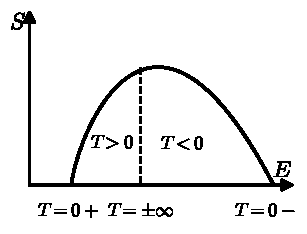
\includegraphics[width=6.5cm]{fig10.pdf}\\[0.3em]{\small 图 10}\end{minipage}\par\nopagebreak

由此可见，负温度的区域并不位于“绝对零度之下”，而是位于“无限大温度之上”.在这种意义下可以说：负温度比正温度“更高”.与这种论断一致的是这样一个事实：当具有负温度的系统同具有正温度的系统(同晶格振动)相互作用时，能量一定是从前一系统转移到后一系统中去的，这一点可以用在§9中用来研究温度不同的物体之间的能量交换的那种方法来证实.

负温度状态可以在晶体的诸原子核磁矩所构成的顺磁系统中具体实现，只要在这种晶体中核自旋相互作用的弛豫时间 $t_2$ 比自旋和晶格之间相互作用的弛豫时间 $t_1$ 小得多(E.~M.~Purcell, R.~V.~Pound, 1951).设晶体在强磁场中受到磁化，然后把磁场方向如此迅速地反过来，以使得自旋“来不及”随着反向.这样就使得系统停留在一个非平衡状态，其能量显然高于 $\overline{E}_n$.经过数量级为 $t_2$ 的时间，它达到一个具有同样能量的平衡状态.如果随后以绝热的方式把磁场移去，就使得系统所停留的状态显然是一个具有负温度的平衡状态.随后在自旋系统和晶格之间交换能量，同时它们的温度变为相等，这将在 $t_1$ 数量级的时间里发生.
